\documentclass[conference]{IEEEtran}

% --- Packages ----------------------------------------------------------------
\usepackage[T1]{fontenc}
\usepackage[utf8]{inputenc}
\usepackage{amsmath}
\usepackage{amssymb}
\usepackage{graphicx}
\usepackage{booktabs}
\usepackage{cite}
\usepackage{listings}
\usepackage{xcolor}
\usepackage{float}
\usepackage{hyperref}
\usepackage{stfloats}

% --- Code listing style ------------------------------------------------------
\definecolor{lightgray}{rgb}{0.95,0.95,0.95}
\definecolor{darkgreen}{rgb}{0.0,0.5,0.0}
\lstset{
	basicstyle=\ttfamily\footnotesize,
	breaklines=true,
	frame=single,
	backgroundcolor=\color{lightgray},
	keywordstyle=\color{blue},
	commentstyle=\color{darkgreen},
}

% --- Title and Authors -------------------------------------------------------
\title{Adaptive Cruise Controller for RC Car Using STM32}

\author{
	\IEEEauthorblockN{Erickson A.\ Mijangos}
	\IEEEauthorblockA{Department of Electrical Engineering\\
		California State University Fullerton, Fullerton, California\\
		eamijangos@csu.fullerton.edu}
	\and
	\IEEEauthorblockN{Dr.\ Mike Turi}
	\IEEEauthorblockA{Department of Electrical Engineering\\
		California State University Fullerton, Fullerton, California\\
		mturi@fullerton.edu}
}

% =============================================================================
\begin{document}
	\maketitle
	
	% --- Abstract ----------------------------------------------------------------
	\begin{abstract}
		This project documents the design and development of an RC Car built from the 
		ground up, as an attempt to implement and test an Adaptive Cruise Control 
		System. Two STM32 Nucleo-Boards from STMicroelectronics are used: the 
		STM32L432KC for the transmitter and the STM32H723ZG for the RC Car. A Python 
		User Interface is developed for controlling the RC Car and performing data 
		acquisition in order to analyze and develop the adaptive cruise controller.
		
		The sensors integrated to the RC Car are the LIS3DH accelerometer and the 
		Garmin LIDAR Lite V3. The accelerometer was used to determine the velocity of 
		the RC Car, and the LIDAR to measure the relative distance to a leading vehicle 
		ahead. During testing, two challenges arose: the velocity calculated by the 
		accelerometer drifted from the true value over time due to sensor noise, and the 
		NRF24L01 lost communication for 1--1.5s every 20ms cycle which affected velocity 
		calculation.
		
		Due to Earth's gravitational influence on the accelerometer, a calibration 
		feature was implemented, but the communication losses made it difficult to 
		confirm its effectiveness. Based on the test results, the adaptive cruise 
		controller could not be fully implemented. Future work includes integrating a 
		Hall Effect sensor and applying a Kalman Filter for sensor fusion to improve 
		velocity accuracy and enable closed-loop speed control.
	\end{abstract}
	
	\begin{IEEEkeywords}
		Adaptive Cruise Control, STM32, PID Controller, LIDAR, NRF24L01, PyQt5, UART.
	\end{IEEEkeywords}
	
	% --- I. Introduction ---------------------------------------------------------
	\section{Introduction}
	\label{sec:intro}
	
	The purpose of this project is to explore electronics, software development,
	sensor integration, numerical analysis, real-time data acquisition, and
	primarily control engineering by building an RC Car from the ground up.
	The RC Car is designed to develop an Adaptive Cruise Controller with data
	acquisition in order to properly implement it. Figure~\ref{fig:blockdiagram}
	shows a high-level overview of the entire project — the RC Car listens and
	sends data back to the transmitter, which is connected to a Python User
	Interface. The RC Car and transmitter communicate using the NRF24L01
	programmable RF module, and the transmitter connects to the computer via USB
	using the UART protocol to send commands and receive data.
	
	% Block diagram — single column, stays on page 1
	\begin{figure}[H]
		\centering
		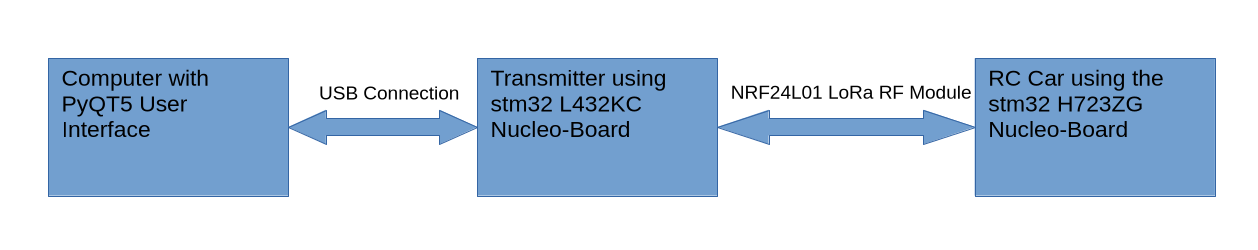
\includegraphics[width=0.48\textwidth]{docs/images/blockDiagrams/blockDiagramHighlLevelProject.png}
		\caption{High-level overview of the project architecture.}
		\label{fig:blockdiagram}
	\end{figure}
	
	The setup of the Transmitter and Python User Interface is shown in
	Figure~\ref{fig:TransmitterUI}, and the RC Car with the transmitter is shown
	in Figure~\ref{fig:TransmitterRC}. The RC Car integrates the LIS3DH
	accelerometer to measure velocity and the Garmin LIDAR Lite V3 to measure
	relative distance.
	
	Based on a simulation study conducted in MATLAB/Simulink at
	CSULB\footnote{Full report available in the project repository:
		\href{https://github.com/eam95/RC_Car_Mark_I/blob/main/docs/EE471\_ACC\_CSULB.pdf}
		{\texttt{EE471\_ACC\_CSULB.pdf}}.}, the Adaptive Cruise Control system is
	designed to autonomously maintain the desired velocity while detecting and
	measuring the relative distance to a leading vehicle ahead. As shown in
	Figure~\ref{fig:ACC_Func}, the relative distance and vehicle speed are
	analyzed to tune the adaptive cruise controller.
	% Put ACC Func figure here so it stays on page 1
	\begin{figure}[H]
		\centering
		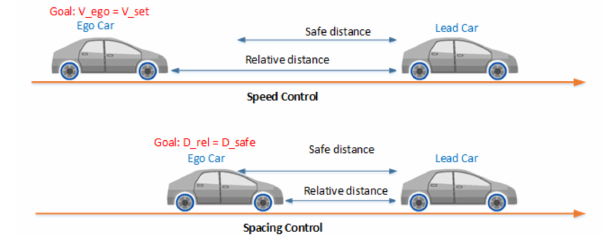
\includegraphics[width=0.45\textwidth]{docs/images/picturesGeneral/ACC_Functionality.png}
		\caption{Speed/Spacing Control to setup Adaptive Cruise Control.}
		\label{fig:ACC_Func}
	\end{figure}
	To implement the adaptive cruise controller in hardware, the Garmin LIDAR
	Lite V3 serves as the primary distance sensor, measuring the relative
	distance between the Ego Car (the RC Car under ACC control) and the Leading
	Car (a second RC Car given a specified motion). The LIS3DH accelerometer
	measures the Ego Car velocity, in which a PID controller can be developed to
	make the RC Car autonomous. The Leading Car will be given a speed with a
	small oscillation to simulate realistic driver behavior, as shown in
	Figure~\ref{fig:ACC_Simu_UI}.
	
	To achieve the simulated behavior of the adaptive cruise controller, the
	control system shown in Figure~\ref{fig:ACC_HighLevel} models the Leading
	Vehicle motion and the Sensor Model, which depends on the relative position
	and velocity of the leading vehicle and the ego vehicle, so it can be fed
	into the ego vehicle plant to predetermine next motion. The input signals
	measured from the relative and ego vehicle parameters used to determine the
	ego vehicle Adaptive Cruise Controller are shown in Figure~\ref{fig:EgoSensorBlock}.
	
	% --- All introduction figures on page 2 -------------------------------------
	\clearpage
	
	% Photos side by side
	\begin{figure*}[t]
		\centering
		\begin{minipage}{0.48\textwidth}
			\centering
			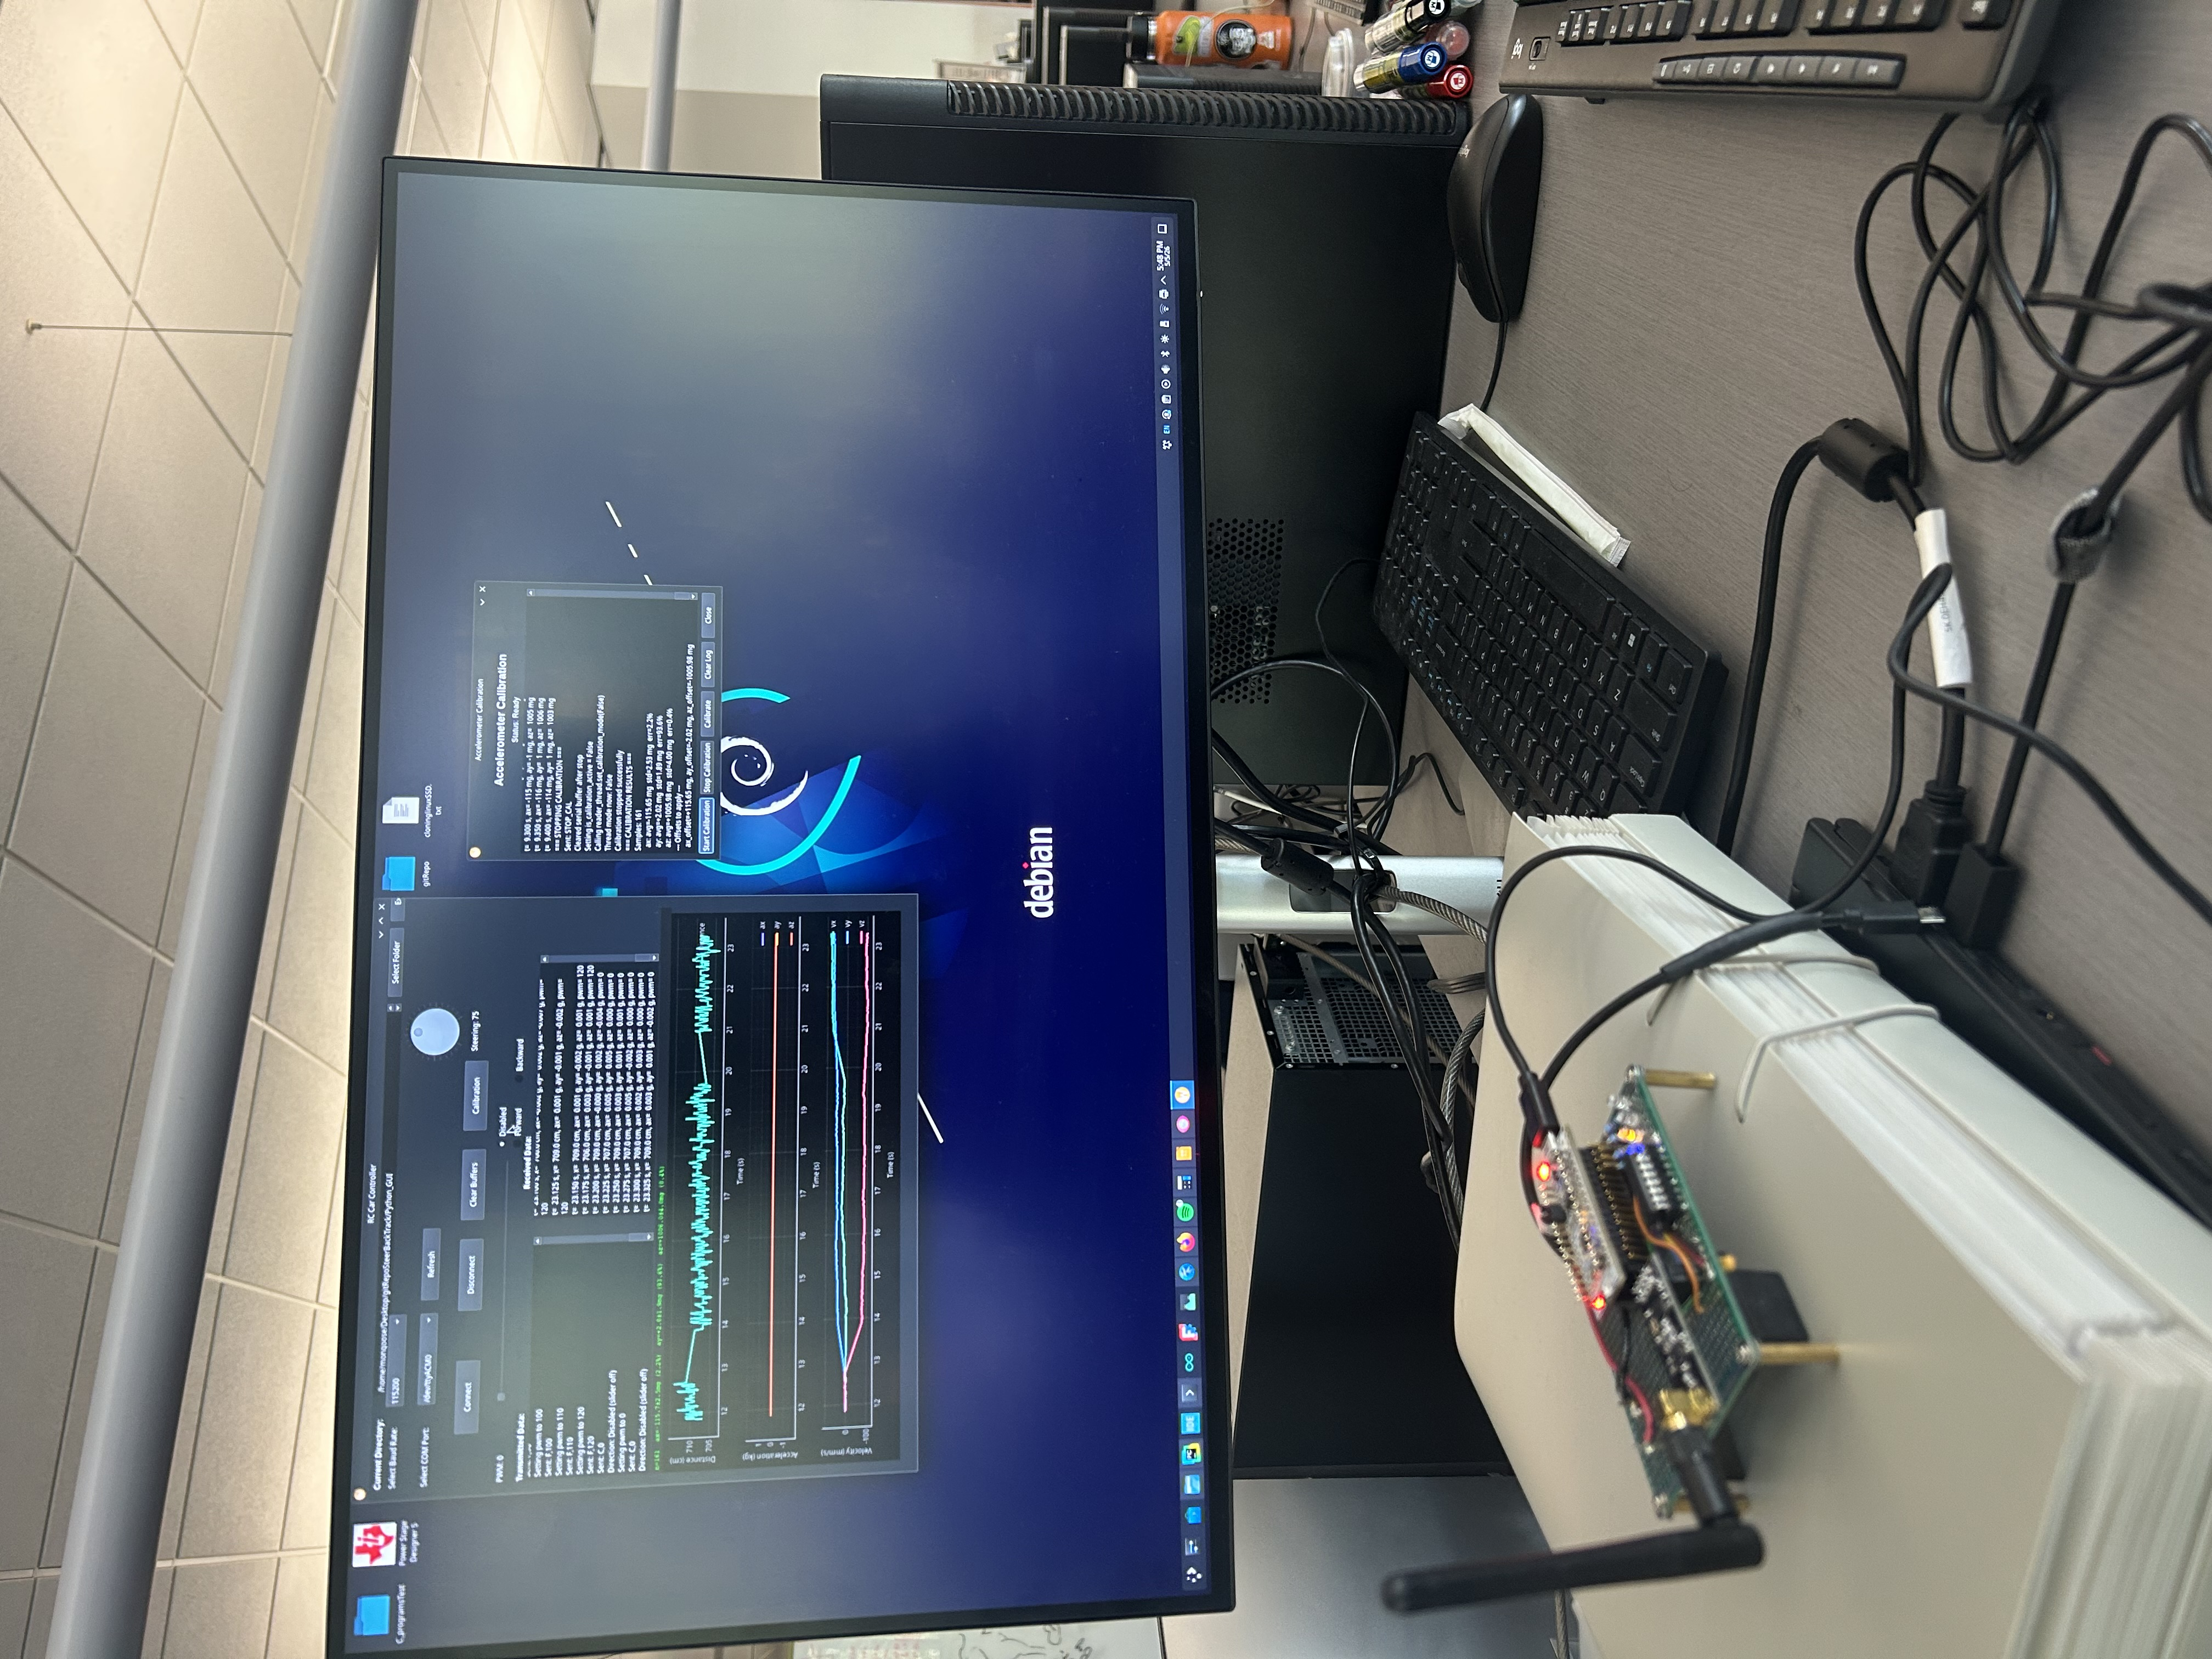
\includegraphics[width=\textwidth, angle=270]{docs/images/picturesGeneral/transmitterAndPythonUserInterface.jpg}
			\caption{The Transmitter connected to the Python user interface.}
			\label{fig:TransmitterUI}
		\end{minipage}
		\hfill
		\begin{minipage}{0.48\textwidth}
			\centering
			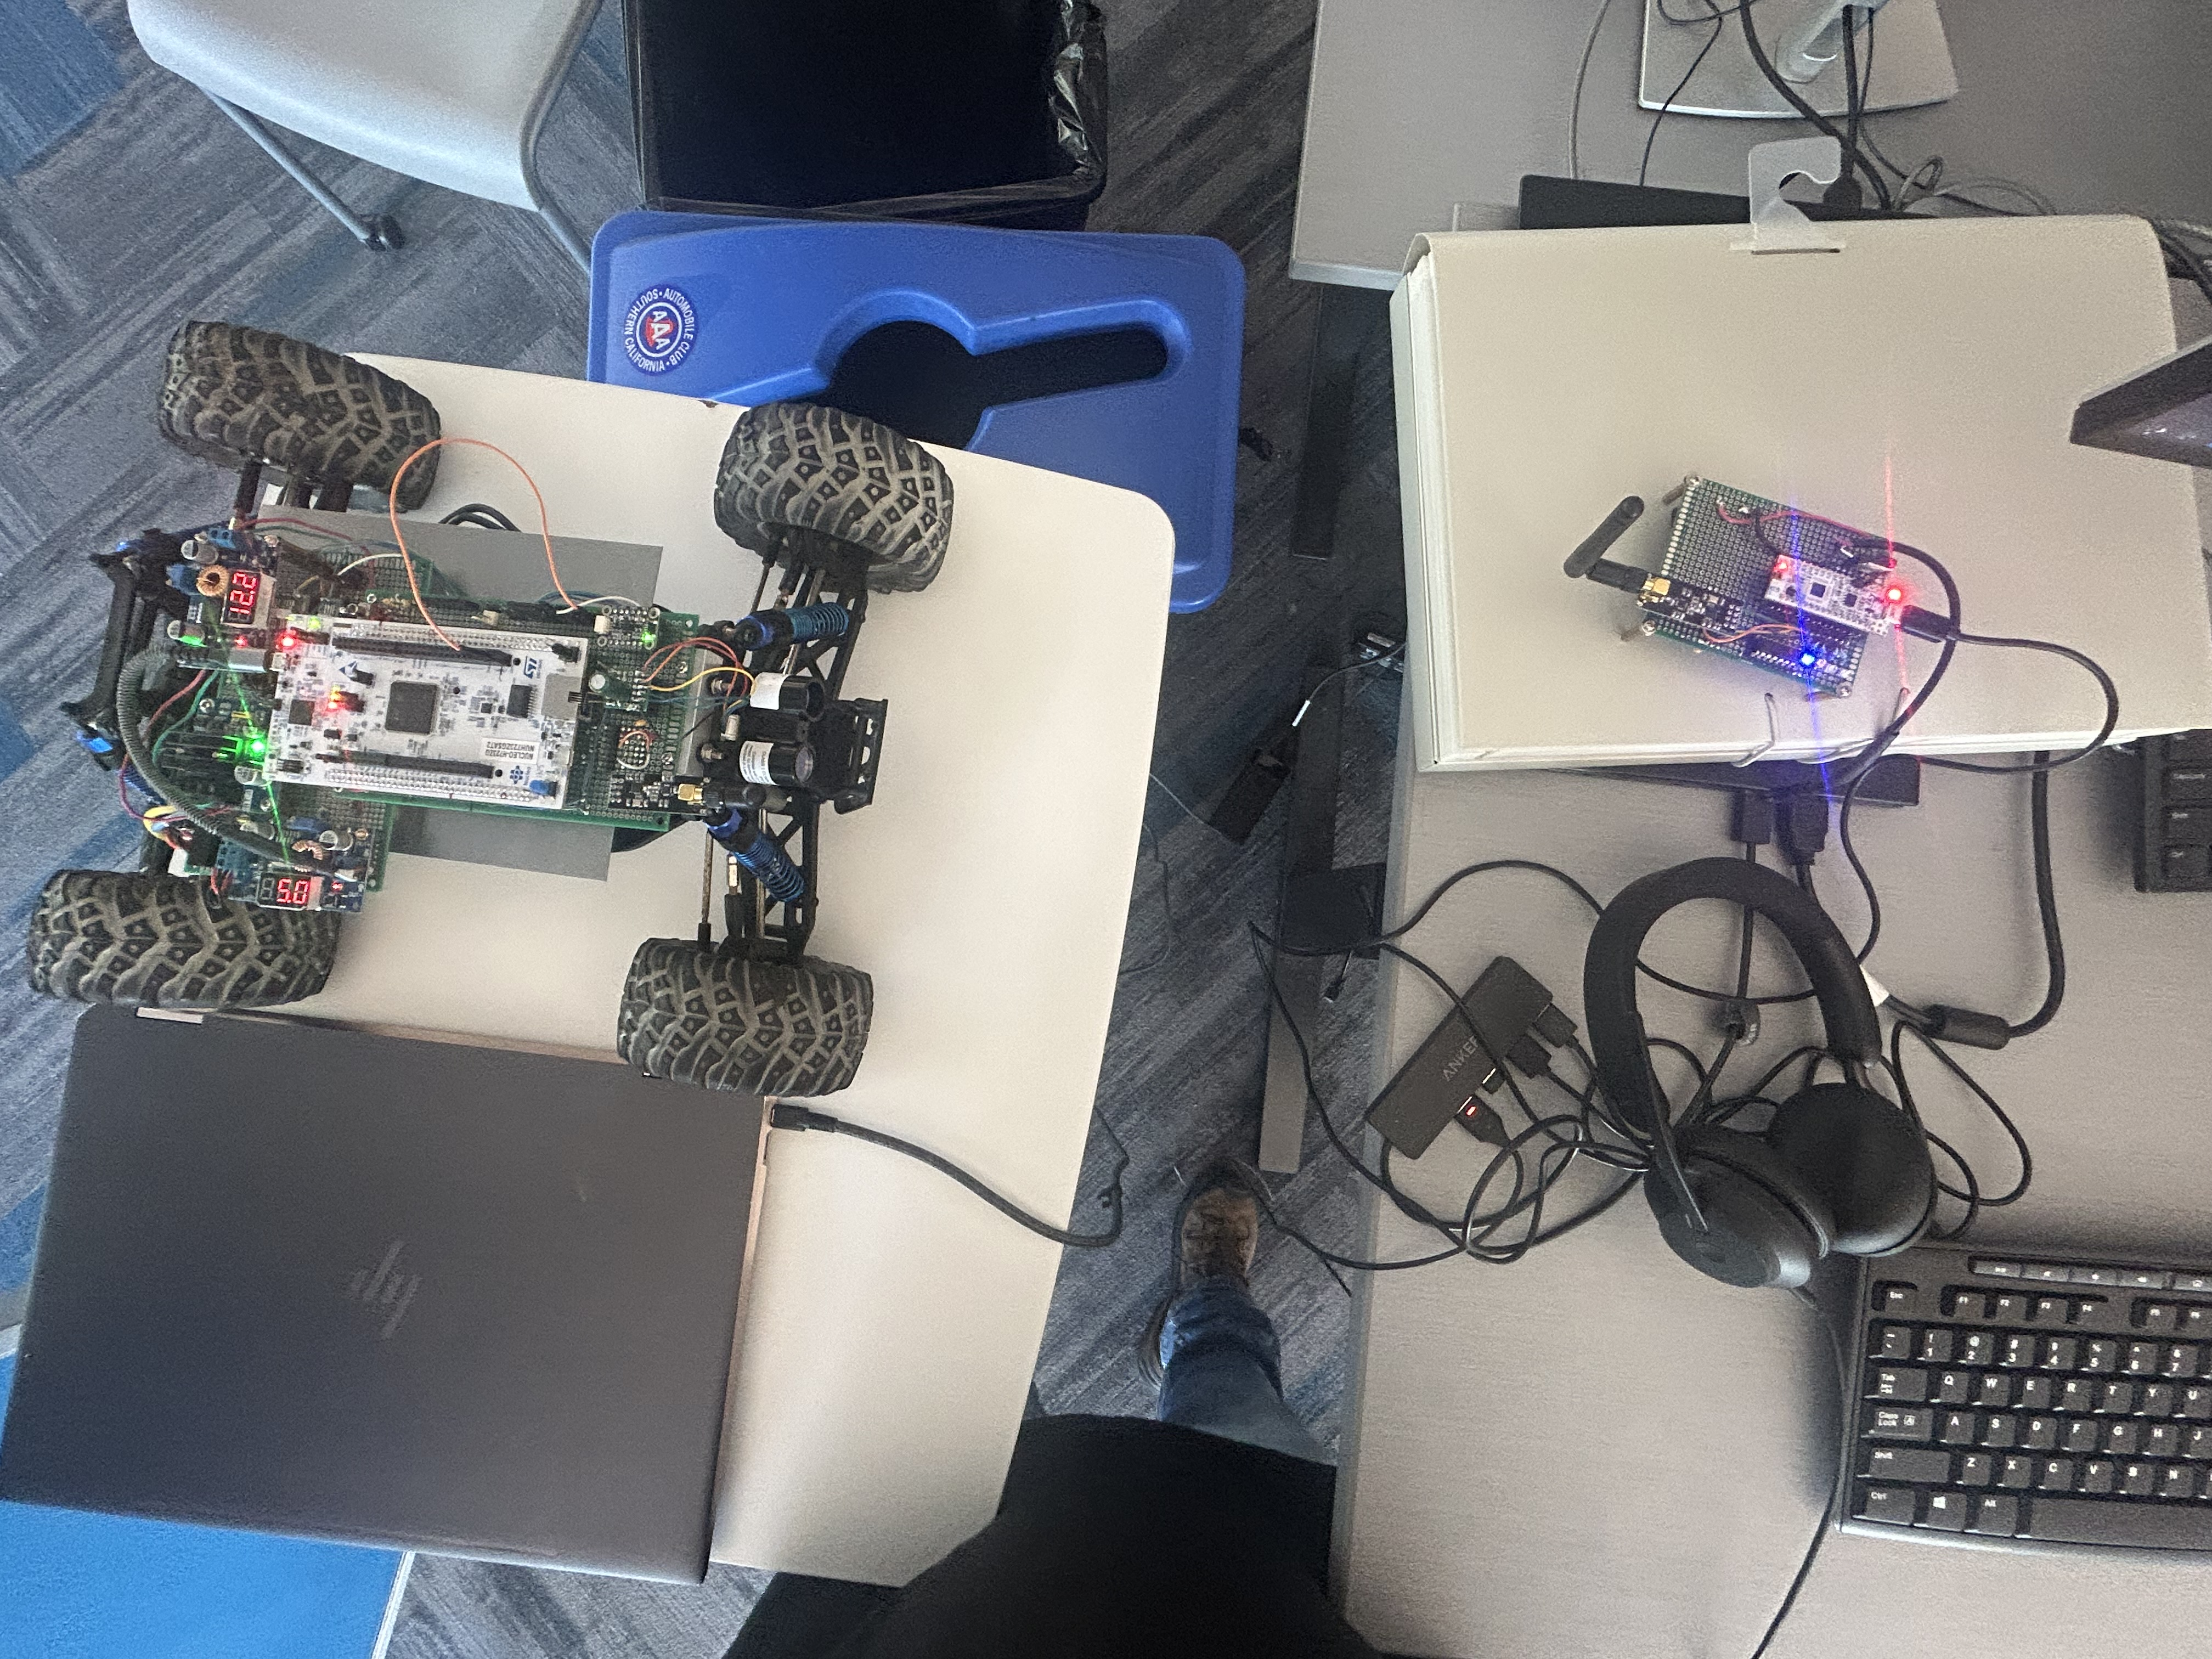
\includegraphics[width=\textwidth, angle=270]{docs/images/picturesGeneral/transmitterAndRC_Car.jpg}
			\caption{The Transmitter and RC Car.}
			\label{fig:TransmitterRC}
		\end{minipage}
	\end{figure*}
	
	% MATLAB Simulink UI
	\begin{figure*}[t]
		\centering
		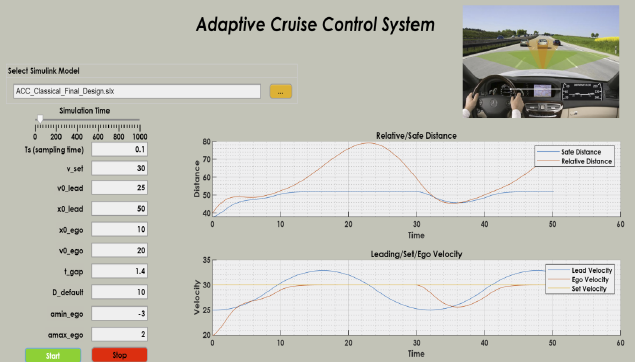
\includegraphics[width=0.9\textwidth]{docs/images/picturesGeneral/ACC_SimulinkModel.png}
		\caption{The User Interface developed in MATLAB and Simulink.}
		\label{fig:ACC_Simu_UI}
	\end{figure*}
	
	% --- ACC model on page 3 ------------------------------------
	\clearpage
	
	% ACC high level model
	\begin{figure*}[t]
		\centering
		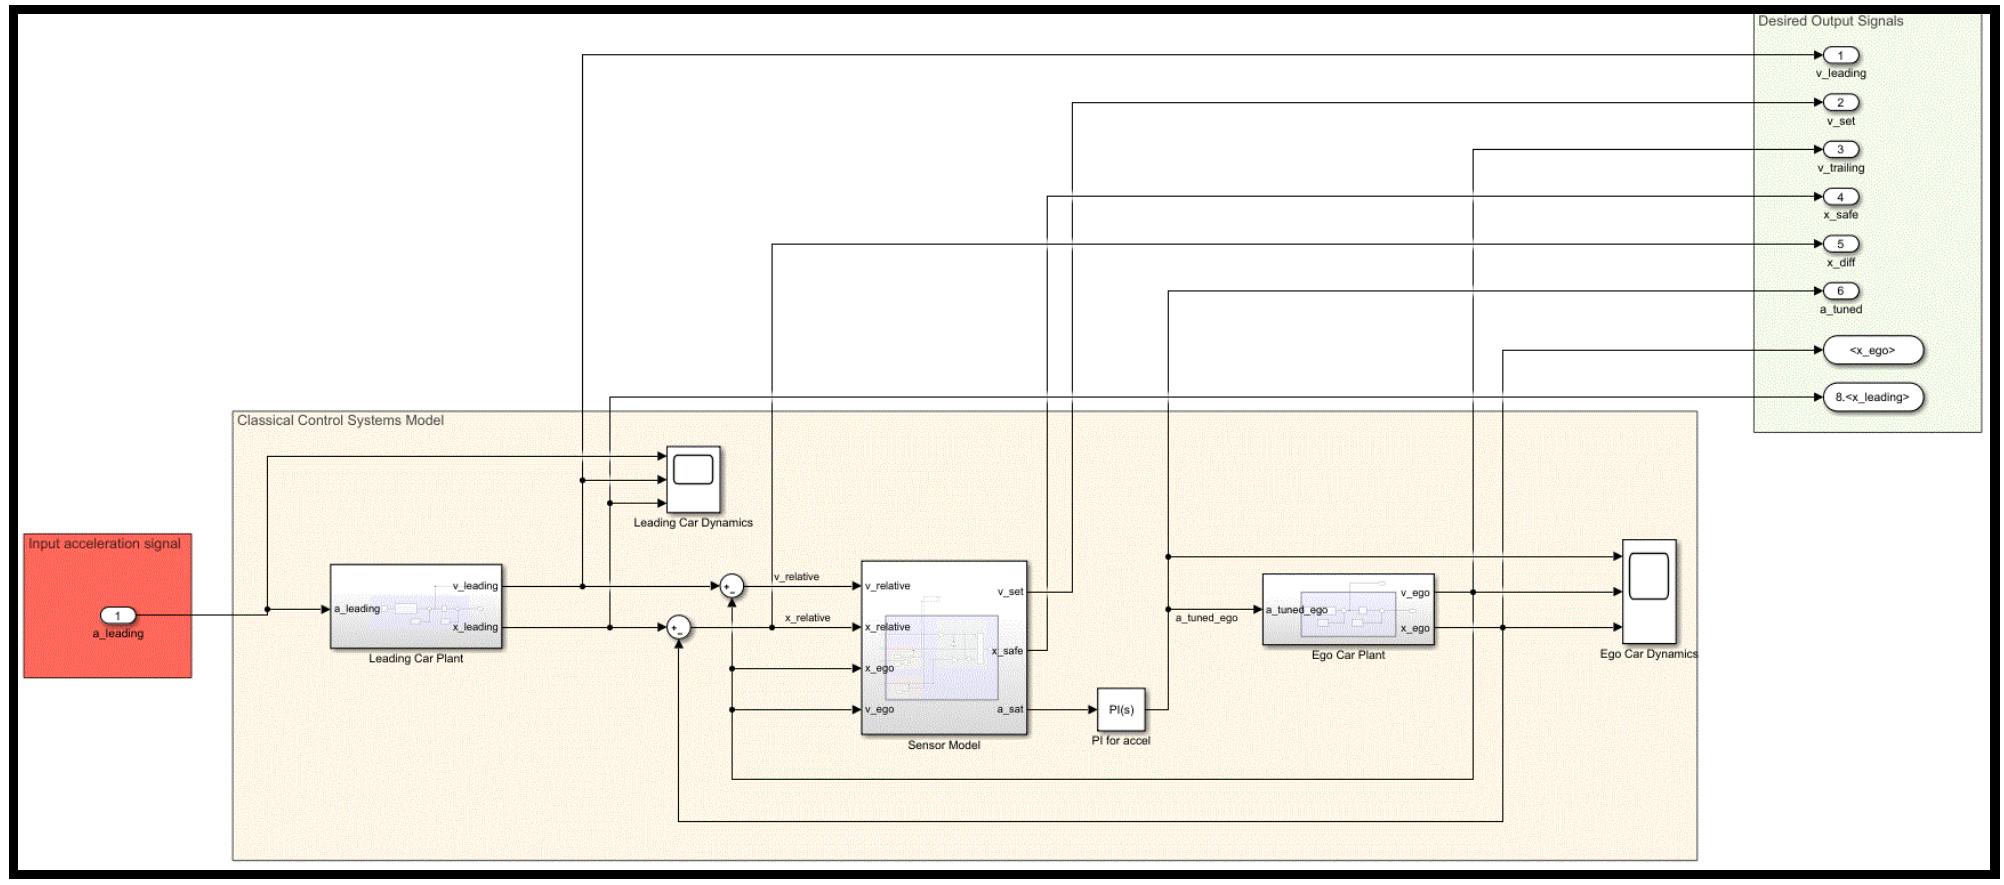
\includegraphics[width=1\textwidth]{docs/images/blockDiagrams/blockDiagramHighlLevelACC_Model.png}
		\caption{High-level overview of ACC model.}
		\label{fig:ACC_HighLevel}
	\end{figure*}
	
	% Ego sensor model
	\begin{figure*}[t]
		\centering
		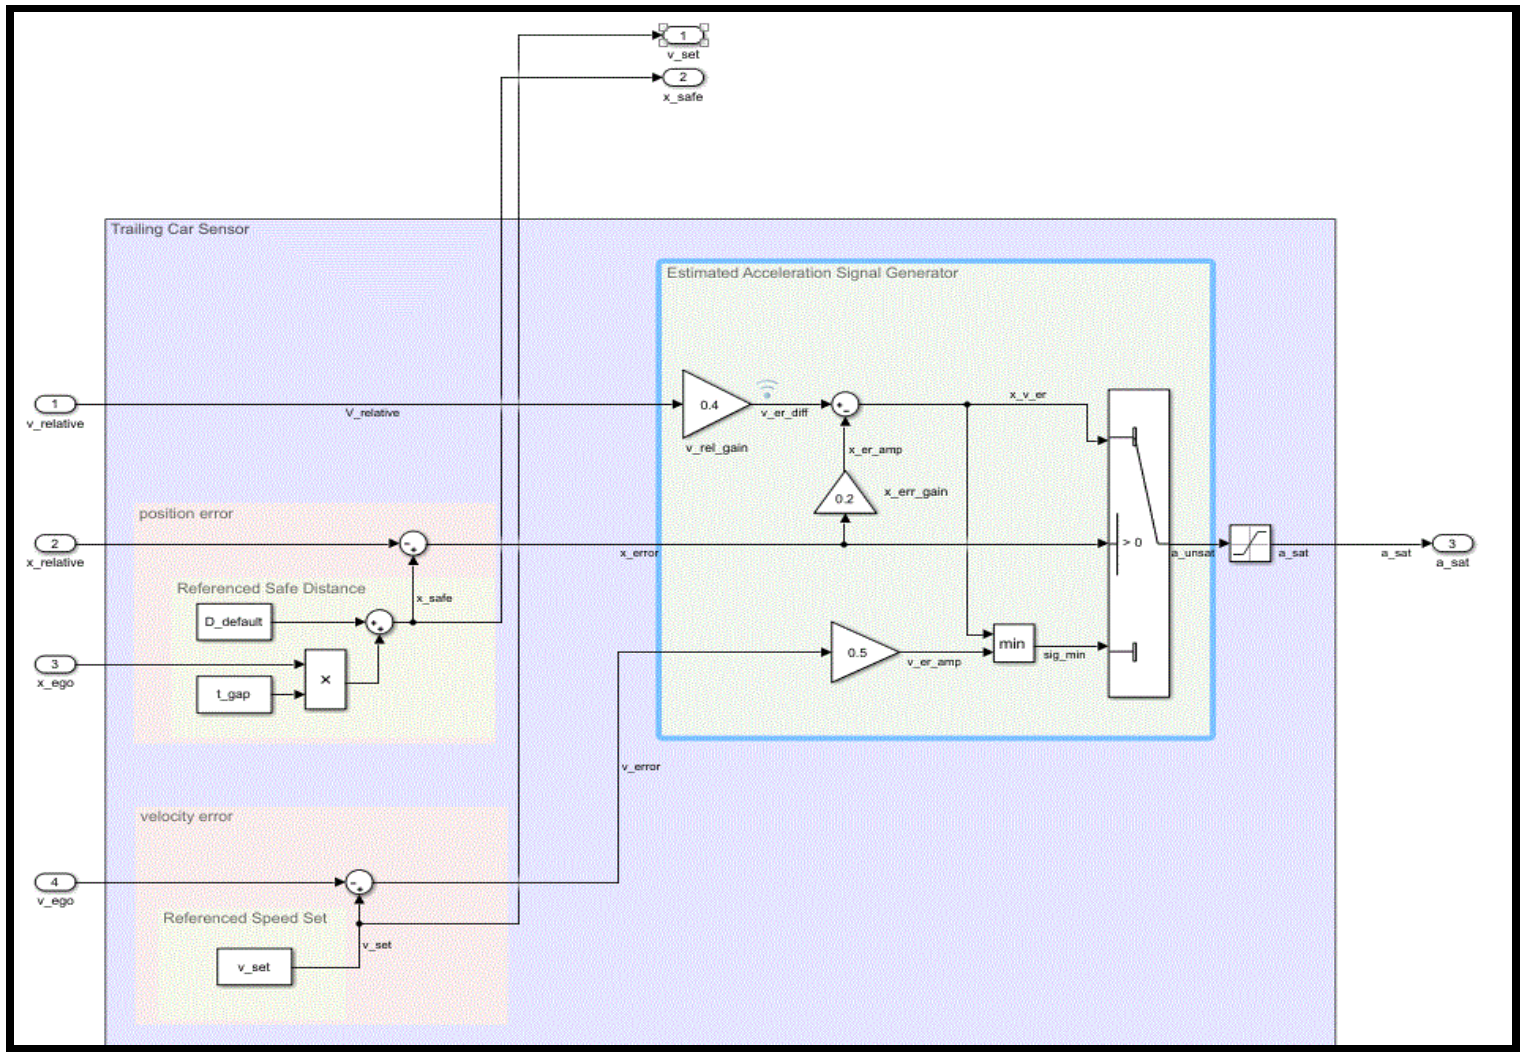
\includegraphics[width=0.85\textwidth]{docs/images/blockDiagrams/EgoSensorModel.png}
		\caption{Block diagram of vehicle plant and derivation for velocity 
			and position motion.}
		\label{fig:EgoSensorBlock}
	\end{figure*}
	
	% --- Continuation And Hardware Architecture on page 4 ------------------------------------
	
	To place the adaptive cruise controller into test, data acquisition with a
	decent sample rate from both the accelerometer and LIDAR are required. To
	analyze and process the signals collected, the Python user interface needs to
	be implemented in order to acquire data in real time so that a proper adaptive
	cruise controller can be implemented.
	
	\section{Hardware Architecture}
	\label{sec:hardware}
	
	\subsection{RC Car Design}
	
	The RC Car uses the STM32H723ZG Nucleo-Board, due to having the 550MHz clock
	speed, to achieve better timer control if necessary, minimize the execution
	time per instruction, accessibility of more peripherals, and the larger system
	RAM to store large amounts of data for testing purposes. The peripherals used
	in this MCU are SPI, USART, I2C, timers, and Direct Memory Access to either
	control sensors and transmit data during development. Figure~\ref{fig:Schematic_RC_Car}
	shows the STM32H723ZG Nucleo-Board integrated with all the sensors and the
	power system section, along with the RC Car with all sensors and modules
	labeled in Figure~\ref{fig:RC_CarLabeled}.
	
	The entire RC Car is powered by a 12V battery, and is divided into subsections
	based on the schematic. On the left, a yellow box shows the MCU along with its
	sensors, and on the right the green box shows the power system and the motor
	driver. The power section is electrically isolated due to the FOD8001 Logic
	Optocouplers and the TMH1205S 2W Traco Isolated DC-DC Converter, which isolate
	the power ground and digital ground on the MCU section. This feature is added
	to troubleshoot, isolate noise that can influence the sensors during data
	transmission, and ensure that if any power section components or modules are
	destroyed it would not destroy the MCU and the sensors.
	
	As labeled in the RC Car schematic, the sensors are mapped to their
	corresponding pins on the MCU along with their communication protocols. The
	NRF24L01 RF module uses the SPI protocol where the data rate is set to
	$\sim$3.9~Mbit/s. According to the NRF24L01 datasheet, the module requires
	130~$\mu$s to switch between RX and TX mode, and including the execution
	timing of the program can add additional time. When bidirectional communication
	was first tested, the bare minimum for reliable communication was found to be
	4ms. To provide reliable bidirectional communication consistently, 10ms is used
	before toggling RX/TX mode. The 10ms toggling time also accounts for the time
	required to read the sensor data and package it for transmission. On the MCU,
	three built-in LEDs are used to track the state of the RC Car firmware.
	Adding the status LEDs helps the user keep track of and troubleshoot the RC Car
	during development.
	\begin{itemize}
		\item \textbf{Yellow LED} — RC Car is in TX mode (sending sensor data to transmitter)
		\item \textbf{Red LED} — Data packet transmitted from RC Car
		\item \textbf{Green LED} — Command received from transmitter for RC Car next action
	\end{itemize}
	
	The remaining two sensors that use the I2C protocol are the LIS3DH
	accelerometer and the Garmin LIDAR Lite V3. The clock speed that the MCU can
	configure for the I2C protocol is either 100kHz or 400kHz. Both sensors are
	clocked at 400kHz, which was confirmed to be reliable when both sensor
	libraries were written. The perfboard that holds the MCU has the wires soldered
	close to the MCU in order to ensure I2C reliability and minimize stray
	capacitance that can affect the rise and fall times of both data and clock
	lines. Both sensors are sampled when the firmware is in the state to transmit
	data to the transmitter, which occurs every 20ms.
	
	With the MCU and sensors isolated from the power section, the FOD8001
	optocouplers and servo motor still need to be powered. With 12V serving as the
	main power source of the RC Car, the MCU, optocouplers, and motor driver need
	to be powered properly by adding voltage regulators and DC/DC converters. The
	optocouplers on the power section still need to be powered at approximately 5V
	so that the PWM pulse can be passed to the motor driver and servo motor.
	
	% RC Car Labeled
	\begin{figure}[H]
		\centering
		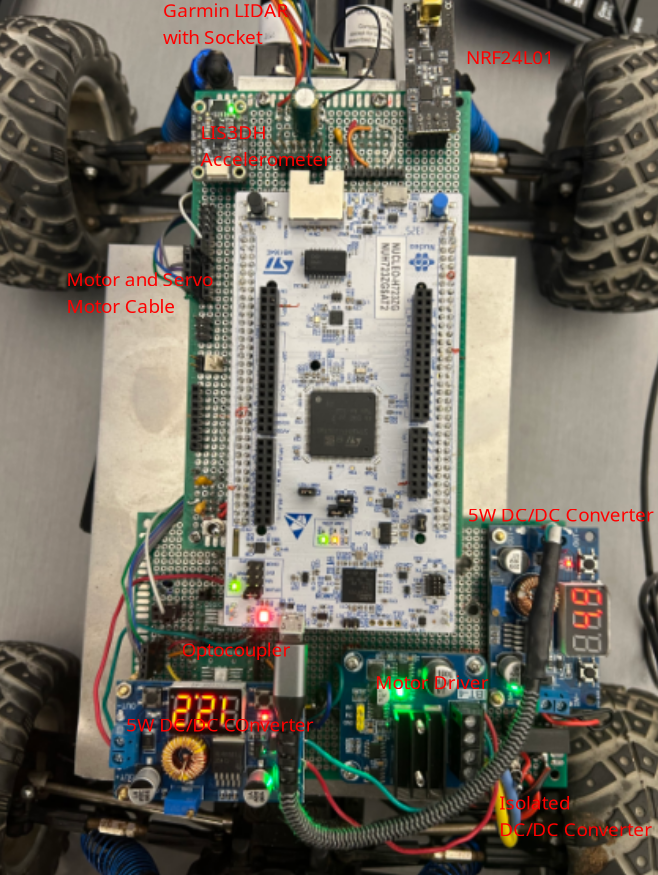
\includegraphics[width=0.3\textwidth]{docs/images/picturesGeneral/RC_CarLabeled.png}
		\caption{RC Car Labeled.}
		\label{fig:RC_CarLabeled}
	\end{figure}
	
	% --- Schematic of RC Car and Transmitter on page 5 ------------------------------------
	\clearpage
	\begin{figure*}[t]
		\centering
		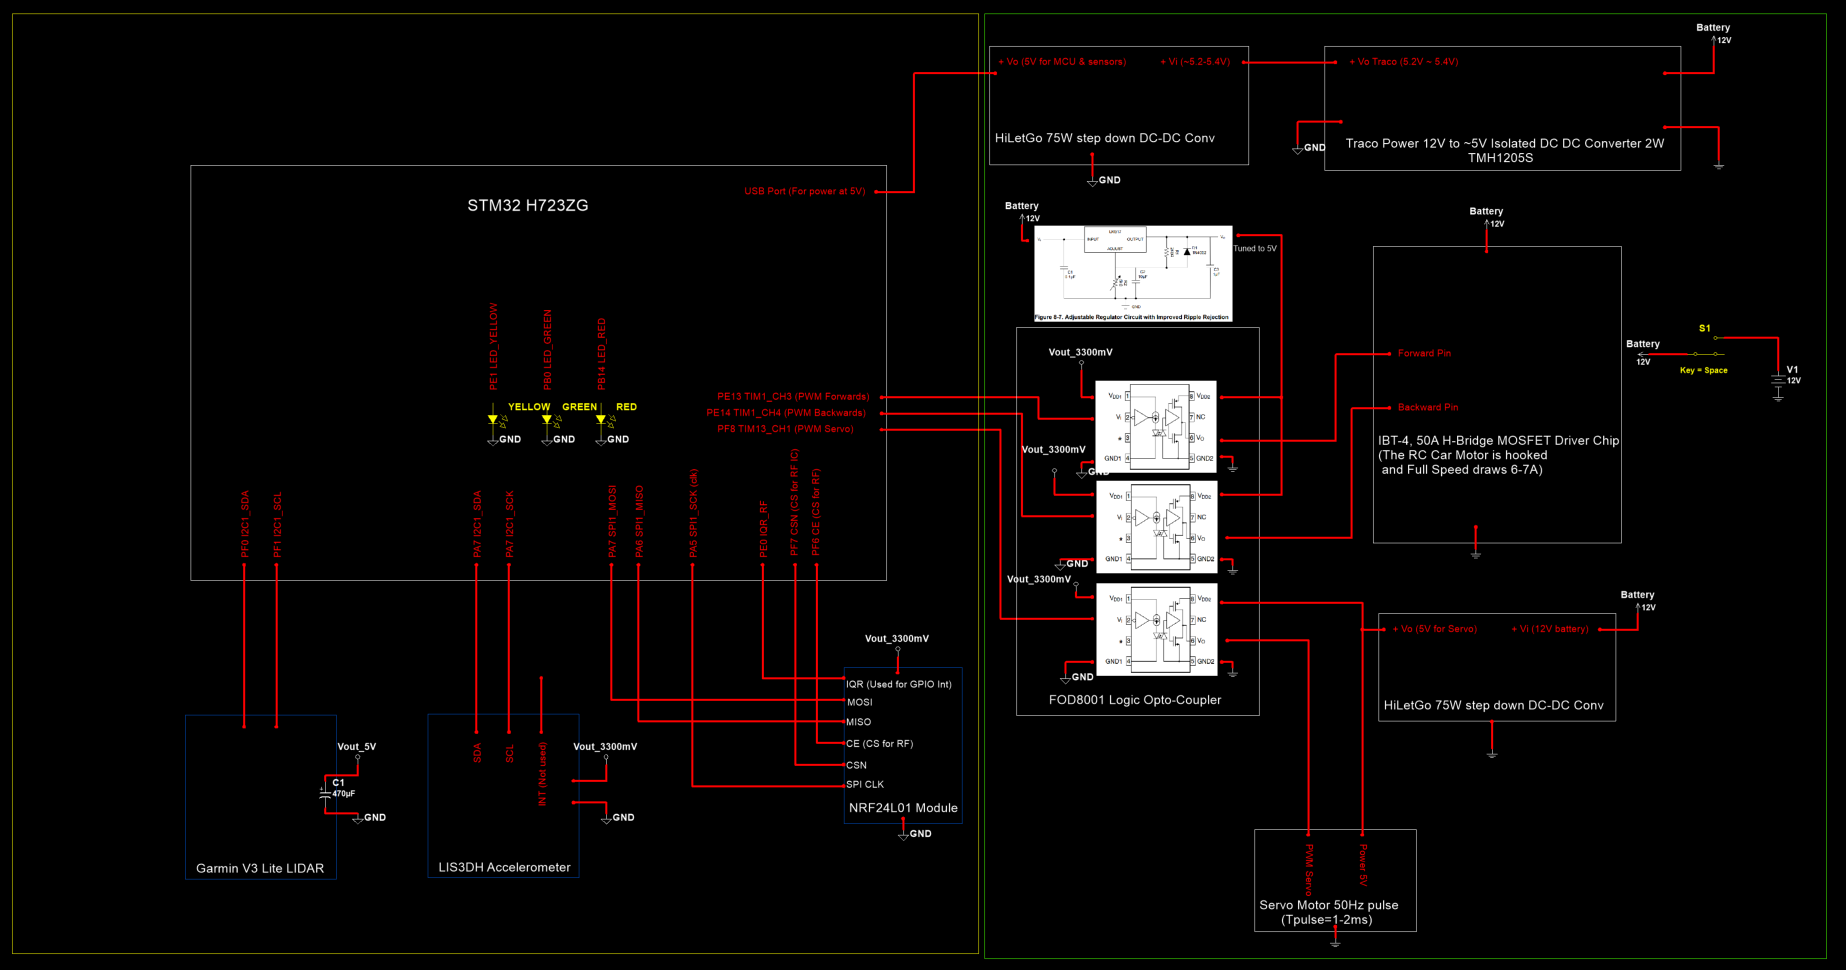
\includegraphics[width=0.95\textwidth]{docs/schematics/RC_Car_Schematic.png}
		\caption{The Schematic of RC Car.}
		\label{fig:Schematic_RC_Car}
	\end{figure*}
	
	% --- Continuation, Transmitter Design, & Firmware Design on page 6 -----------
	Two of the optocouplers responsible for passing the PWM pulses to the MOSFET
	motor driver are powered by the LM317 voltage regulator, which can be tuned to
	5V based on the adjustable circuit from the Texas Instruments datasheet as
	shown in the schematic. Both the third optocoupler and servo motor are powered
	by the 75W HiLetgo DC/DC stepdown converter. Although both the third
	optocoupler and servo motor could be powered by the LM317, this was not done
	due to concerns that it would heat up and go into thermal runaway. The servo
	draws approximately 500--700mA when manually tested with a 5V supply along with
	a function generator generating a PWM signal pulsing within 1--2ms, with a
	period of 20ms (PWM frequency of 50Hz). Since the LM317 drops the 12V to 5V,
	it would have a 7V drop across it, and if more current is drawn it would
	dissipate more heat. As a result, it is a safer route to use the 75W HiLetgo
	DC/DC stepdown converter to power the optocoupler along with the servo motor.
	
	The 75W HiLetgo DC/DC stepdown converter can display the input and output
	voltage it is provided. The battery can be monitored by checking the HiLetgo
	DC/DC converter that is attached to the servo motor and third optocoupler by
	toggling the output push button. The Traco isolated DC/DC converter steps down
	to approximately 5.2V--5.4V from the 12V battery, but a HiLetgo DC/DC
	converter is added between the output of the isolated DC/DC converter and the
	MCU so that it can be tuned to 5V. It can be powered by the isolated DC/DC
	converter, but according to the schematic of the H723ZG Nucleo-Board, the
	Micro-USB port has a zener diode to clamp the supply voltage of the entire
	board to 5V, making it safer to tune it at 5V. When the battery runs low, the
	bare minimum voltage that can be supplied to the MCU to work properly is 4.6V
	before it powers off and becomes unreliable.
	
	\subsection{Transmitter Design}
	
	Compared to the RC Car, the schematic of the transmitter is simpler as shown
	in Figure~\ref{fig:Schematic_Transmitter}, along with the actual labeled
	transmitter in Figure~\ref{fig:Labeled_Transmitter}. The Nucleo-L432KC board
	was chosen for the transmitter due to its small Arduino Nano-like size, and the
	maximum clock speed of 80MHz. The performance does not need to be as robust as
	the Nucleo-H723ZG board since it primarily toggles every 10ms between RX/TX
	mode, and USART interrupts are used to receive commands from the Python User
	Interface and transmit data received from the RC Car back to the User
	Interface. The transmitter is connected to the computer to transmit and receive
	data using the UART protocol with a baud rate of 115200~bits/s.
	
	% Transmitter Labeled
	\begin{figure}[H]
		\centering
		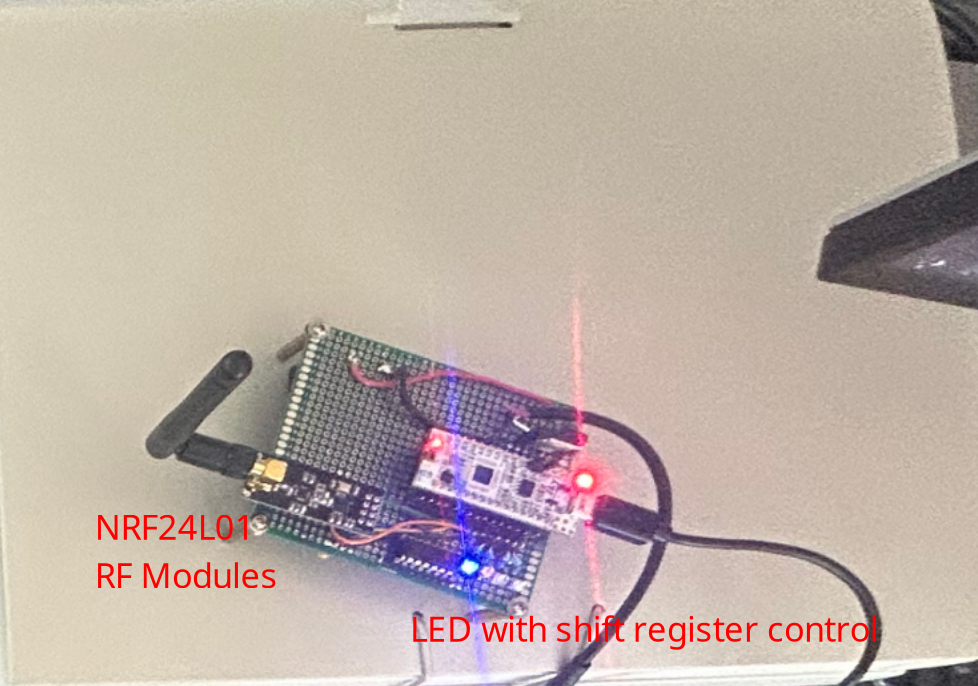
\includegraphics[width=0.35\textwidth]{docs/images/picturesGeneral/transmitterZoomedIn.png}
		\caption{Transmitter Labeled.}
		\label{fig:Labeled_Transmitter}
	\end{figure}
	
	\clearpage
	\begin{figure*}[t]
		\centering
		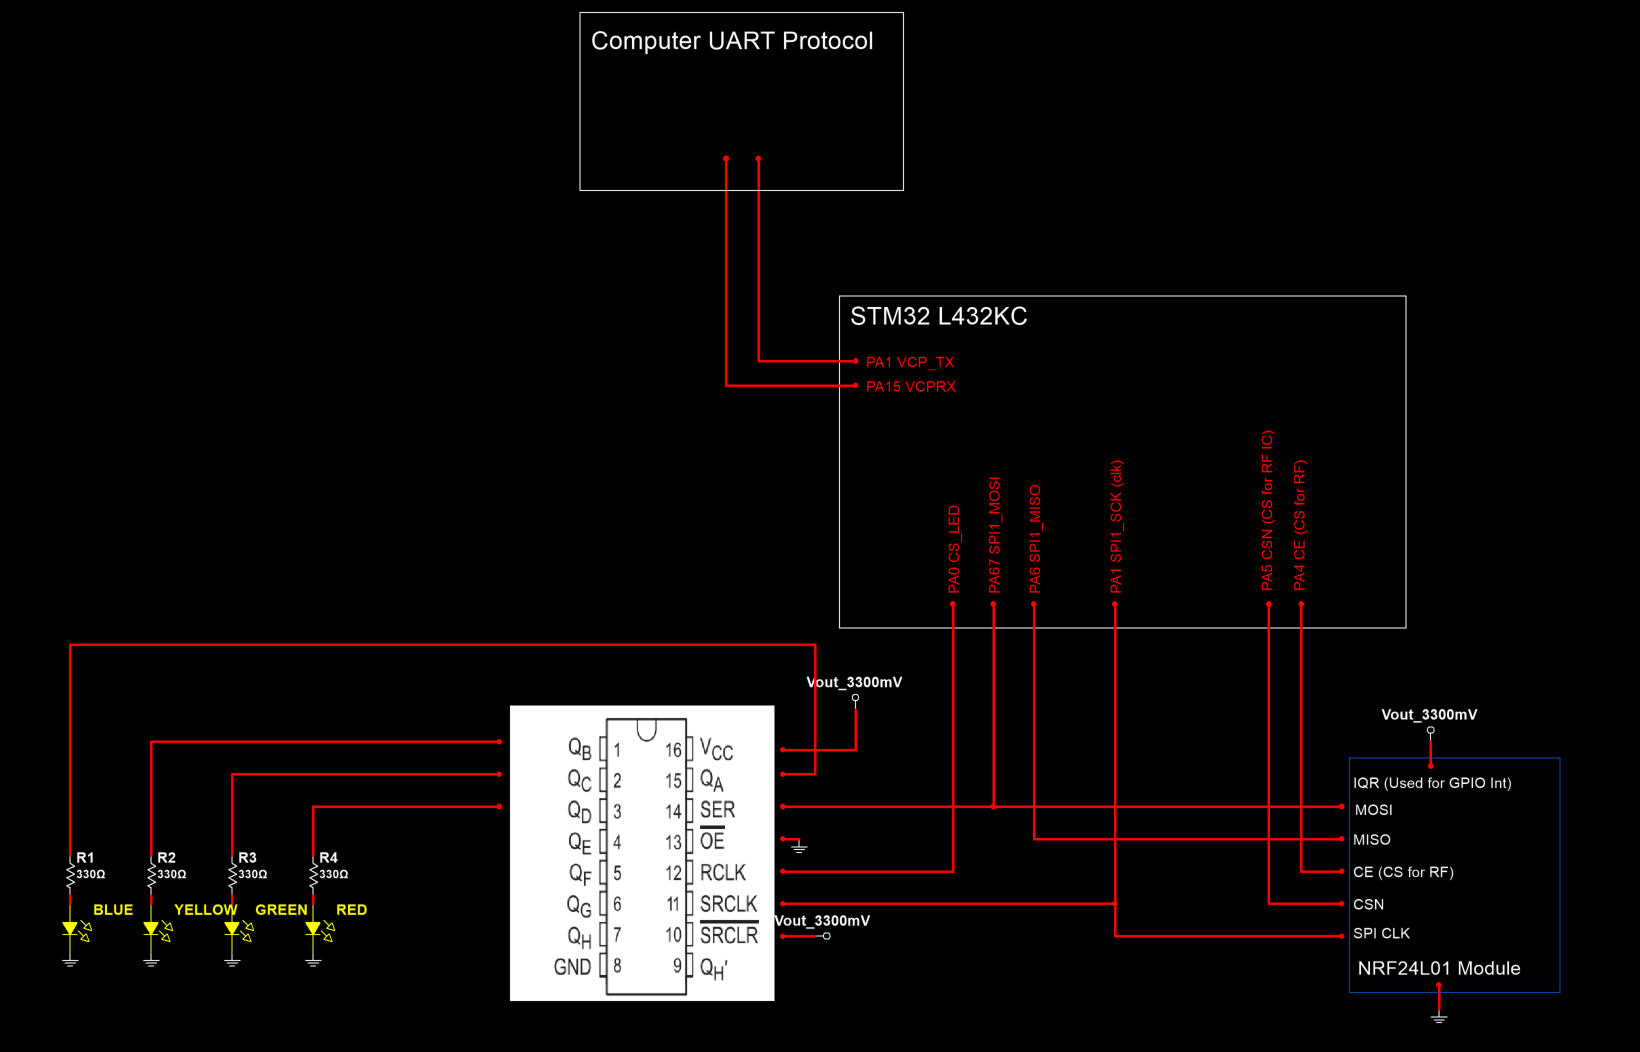
\includegraphics[width=0.95\textwidth]{docs/schematics/TransmitterSchematic.png}
		\caption{The Schematic of Transmitter.}
		\label{fig:Schematic_Transmitter}
	\end{figure*}
	
	Along with the NRF24L01 RF module, a shift register is added to control four
	status LEDs where:
	\begin{itemize}
		\item \textbf{Blue LED} — Transmitter is in RX mode (listening for RC Car data)
		\item \textbf{Yellow LED} — Transmitter is in TX mode (sending command to RC Car)
		\item \textbf{Red LED} — Data packet received from RC Car
		\item \textbf{Green LED} — Command received from Python GUI and ready to transmit
	\end{itemize}
	Adding the status LEDs helps the user track the actions of the transmitter for
	troubleshooting and development.
	
	
	\section{Firmware Design}
	\label{sec:firmware}
	\subsection{RC Car Firmware Design}
	
	Based on the hardware integration of the RC Car, the firmware is designed as a
	Finite State Machine (behaving primarily as a Mealy State Machine where the
	next state varies based on both the current state and inputs). The heart of the
	firmware is Timer 3, which toggles between RX/TX mode and determines the next
	action based on the inputs received during any current state. Figure~\ref{fig:FSM_RC_Car}
	shows the RC Car Finite State Machine logic, where the Timer 3 periodic
	interrupt drives the communication toggling at the center of the diagram. To
	simplify the logic further, pseudocode is added to conditionally determine the
	RC Car's next action.
	
	The movement of the RC Car, including the forward, backward, coast, brake, and
	steer states, varies based on the next state variable, which is determined by
	the command received in the Receive state. If the RC Car is in disable mode,
	it will remain in coast mode; the next state variable will be marked as coast
	state and it will not transmit data back to the transmitter. In the Transmit
	state there is a stopStateFlag which keeps the RC Car disabled — if
	the next state is marked as wait state, it signals the RC Car to remain
	stationary and not transmit sensor data.
	
	When the RC Car receives either forward, backward, or steering commands, it
	will begin transmitting sensor data. During the Receive state for the entire
	10ms window, it remains in a polling state until a command is received from the
	NRF24L01 RF module. If a command is received, the current state is marked to
	get sensor data, and the next state after acquiring sensor data is set to the
	RC Car action, which can be forward, backward, or steering. In the get sensor data state, it checks stopStateFlag if set to
	zero, it can begin acquiring data from the sensors. This flag was added due to
	the calibration feature for calibrating the accelerometer.
	
	\begin{figure*}[t]
		\centering
		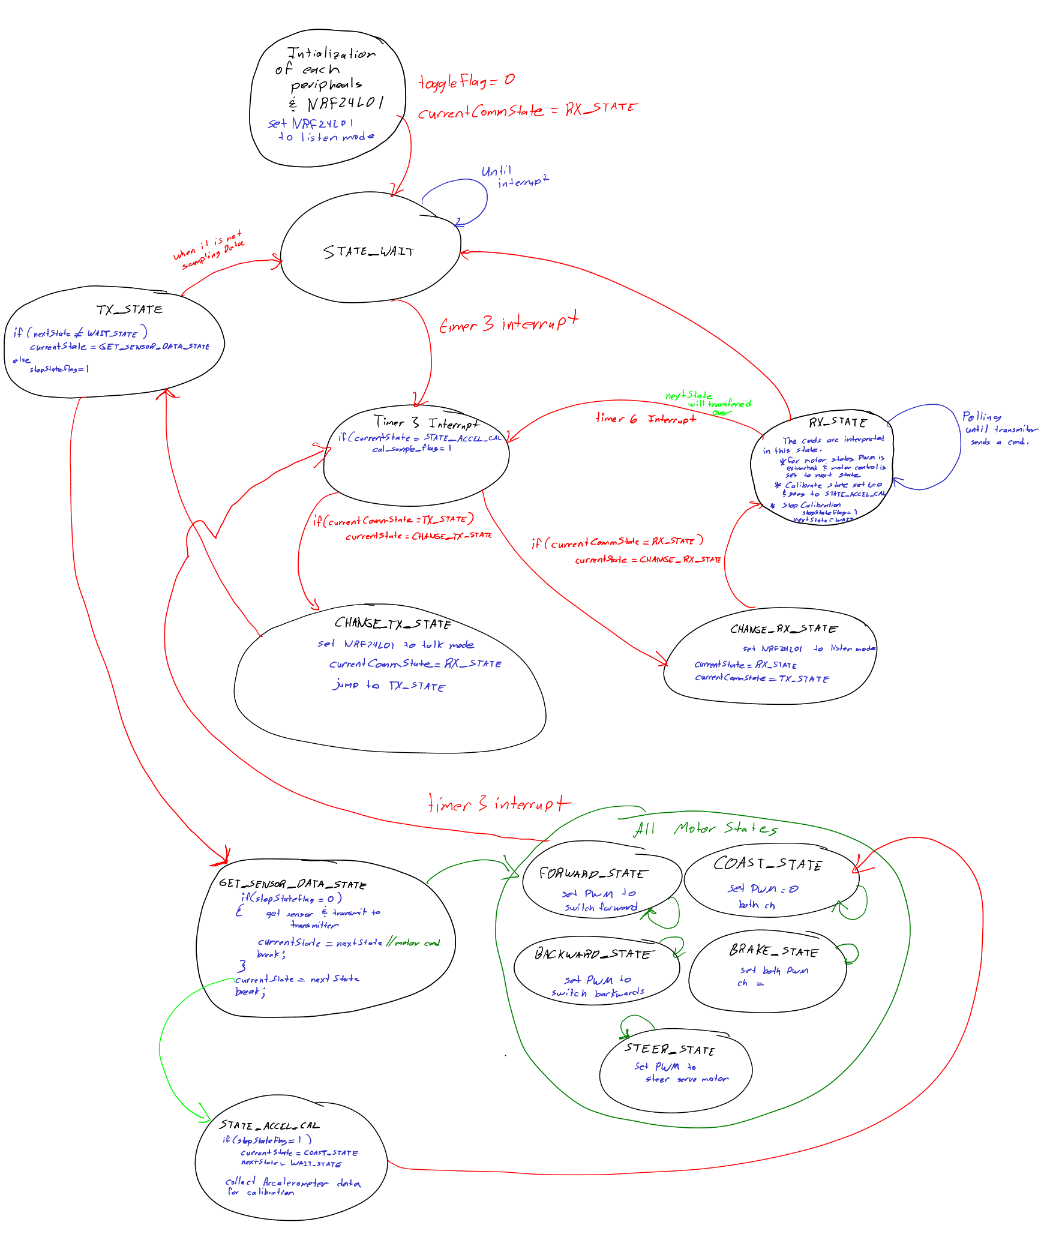
\includegraphics[width=1.00\textwidth]{docs/images/blockDiagrams/RC_CarStateDiagram.png}
		\caption{The finite state machine of the RC Car.}
		\label{fig:FSM_RC_Car}
	\end{figure*}
	\clearpage
	 The difference is that the get sensor data state packages the data in a 32-byte format in the
	following notation:
	\begin{center}
		\texttt{timestamp\_ms,distance\_cm,ax\_mg,ay\_mg,az\_mg\textbackslash n}
	\end{center}
	Whereas the calibration format excludes the LIDAR measurement in the following
	notation:
	\begin{center}
		\texttt{timestamp\_ms,ax\_mg,ay\_mg,az\_mg\textbackslash n}
	\end{center}
	
	\begin{figure*}[t]
		\centering
		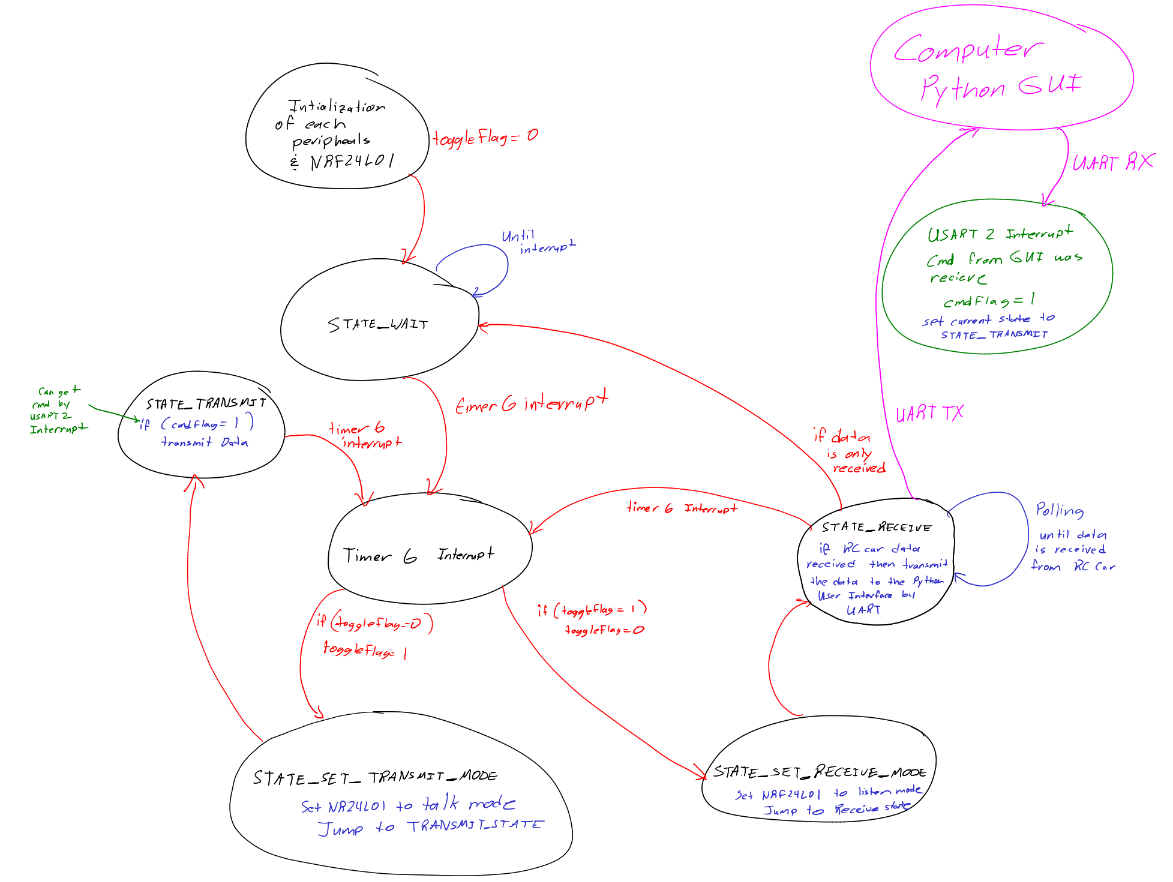
\includegraphics[width=0.80\textwidth]{docs/images/blockDiagrams/transmitterStateDiagram.png}
		\caption{The finite state machine of the Transmitter.}
		\label{fig:FSM_Transmitter}
	\end{figure*}
	
	The calibration state was added since the accelerometer measures Earth's
	gravity, and since a change of motion is desired, the accelerometer data is
	transmitted to calculate the average offset per axis.
	
	\subsection{Transmitter Firmware Design}
	
	The transmitter finite state machine operates in a similar fashion
	(Figure~\ref{fig:FSM_Transmitter}), with the difference of only listening for
	data and transmitting when a USART interrupt occurs at a baud rate of
	115200~bits/s. The USART interrupt signals the MCU that a command has been
	received from the Python User Interface, and the transmitter prepares to
	transmit the command when it switches to the transmit state. When data is
	received during the receive state, it forwards the received data to the Python
	User Interface.
	
	% --- IV. Python GUI ----------------------------------------------------------
	\section{Python Graphical User Interface}
	\label{sec:software}
	
	The transmitter forwards commands to the RC Car and receives data from the RC
	Car under the Python User Interface, as shown in Figure~\ref{fig:PythonUI_Intro}.
	The packages used for the user interface are PyQt5, PyQtGraph for the
	real-time plots, and PySerial to perform UART communication between the user
	interface and the transmitter. The actions performed are displayed in two text
	boxes: the Transmitted Data Box, which shows which buttons were pressed and the
	commands sent to the transmitter, and the Received Data Box, which displays the
	data received from the transmitter. Similarly, the calibration window has a
	text box to display both actions and data received based on the buttons pressed.
	
	In order to display the text box and plot data in real time, the user interface
	uses QThread, imported from the PyQt5 package, otherwise the user
	interface would not respond. The current state diagram does not include the
	logic for determining whether the data is a full measurement (all sensors) or
	accelerometer-only data (for calibration), but the functionality remains the
	same as shown in Figure~\ref{fig:PythonThreadingStateDiagram}. As mentioned in
	the firmware section, the Disable button ensures the RC Car remains stationary
	and will collect data when the steering dial is moved, or when either the
	Forward or Backward radio button is selected with the PWM slider adjusted to
	control speed.
	
	\clearpage
	\begin{figure*}[t]
		\centering
		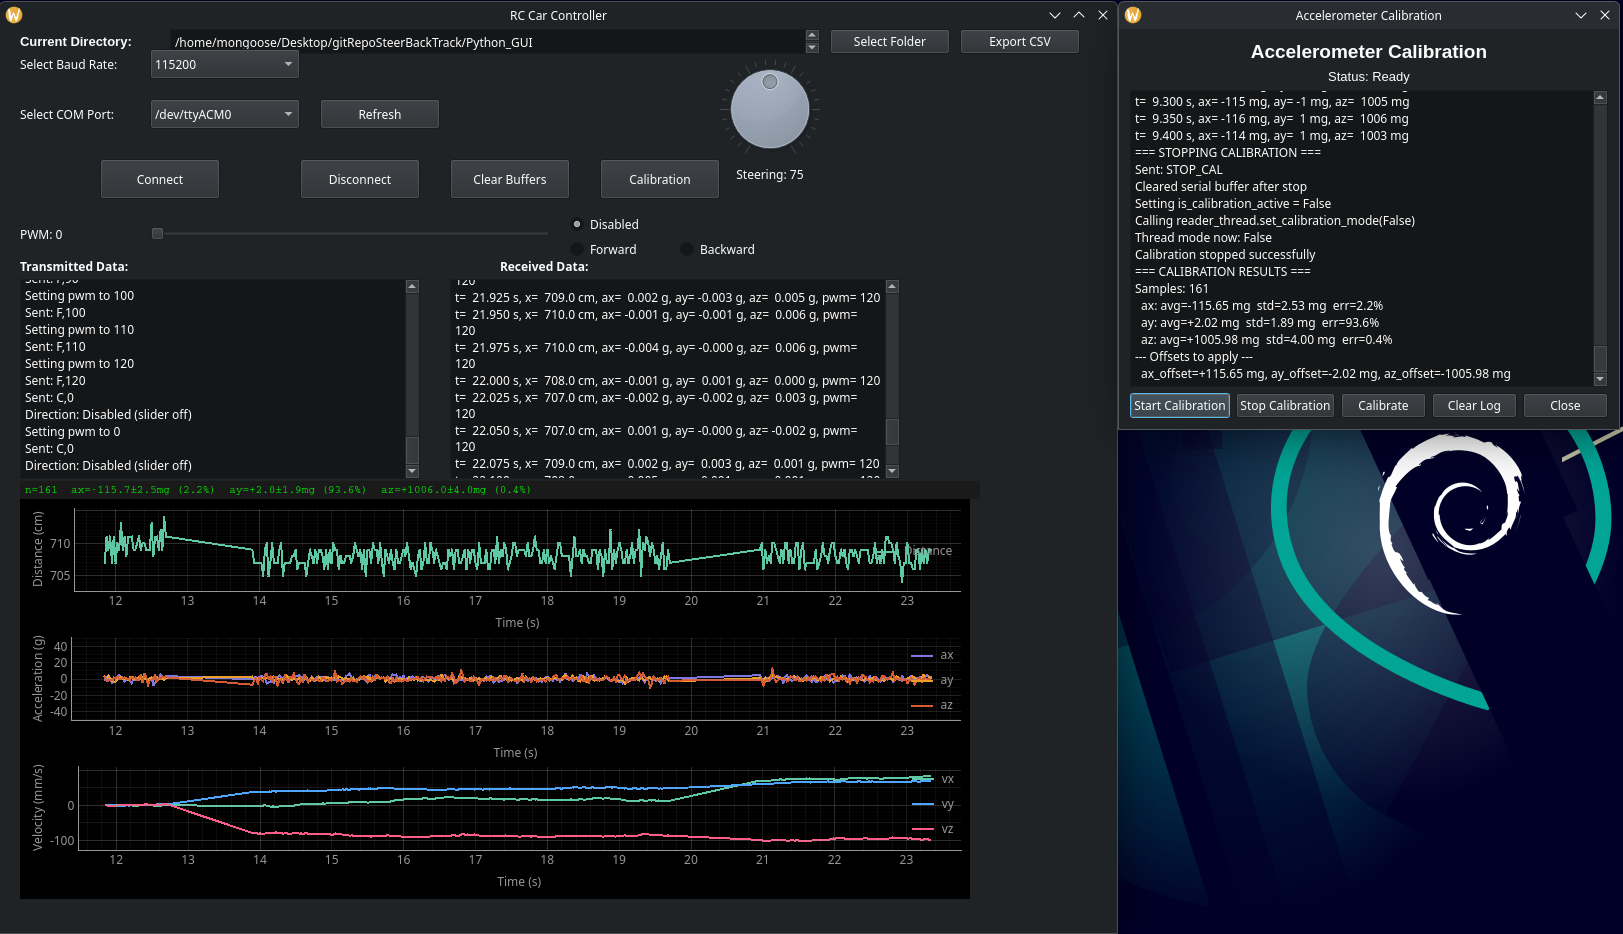
\includegraphics[width=0.85\textwidth]{docs/images/picturesGeneral/PythonGUI.png}
		\caption{The Python User Interface including the Calibration window.}
		\label{fig:PythonUI_Intro}
	\end{figure*}
	\begin{figure*}[t]
		\centering
		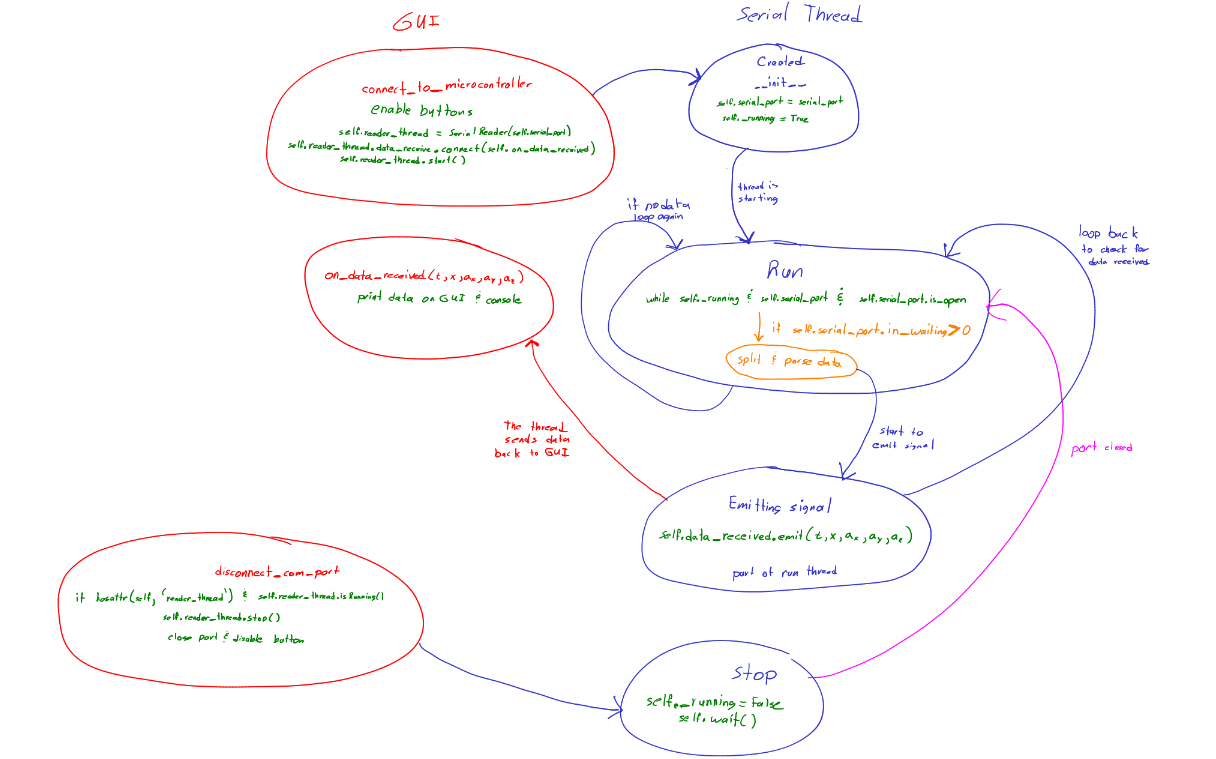
\includegraphics[width=0.68\textwidth]{docs/images/pythonGUI/DisplayDataTextBoxThreadStateDiagram.png}
		\caption{The state diagram for the threading feature when data is received from the transmitter.}
		\label{fig:PythonThreadingStateDiagram}
	\end{figure*}
	
	% --- V. Results --------------------------------------------------------------
	\section{Experimental Results}
	\label{sec:results}
	
	With the RC Car, transmitter, and Python User Interface developed, the RC Car
	was tested to confirm it responds to commands and that data is collected and
	displayed on the User Interface. Figure~\ref{fig:TestDrive} shows the RC Car
	during the first test drive based on a 30-second video recording. Based on the
	recording, no obstacle or wall was detected by the LIDAR throughout the test
	drive, so the distance measurement was unreliable since the maximum range the
	LIDAR can read is up to 40m. All axes of acceleration were acquired, and it can
	be noted that acceleration measurements from the accelerometer are in mg
	(1000mg = 1g). The orange signal is the Z-axis acceleration, which is
	typically close to 1000mg, indicating Earth's gravitational influence on the
	accelerometer. Since the CSV file was not exported at the time of testing, it
	is difficult to zoom in on the X and Y acceleration components, but the video
	showed the velocity for both components zoomed in Figure~\ref{fig:TestDriveZoomedVelocity}.
	
	\begin{figure*}[t]
		\centering
		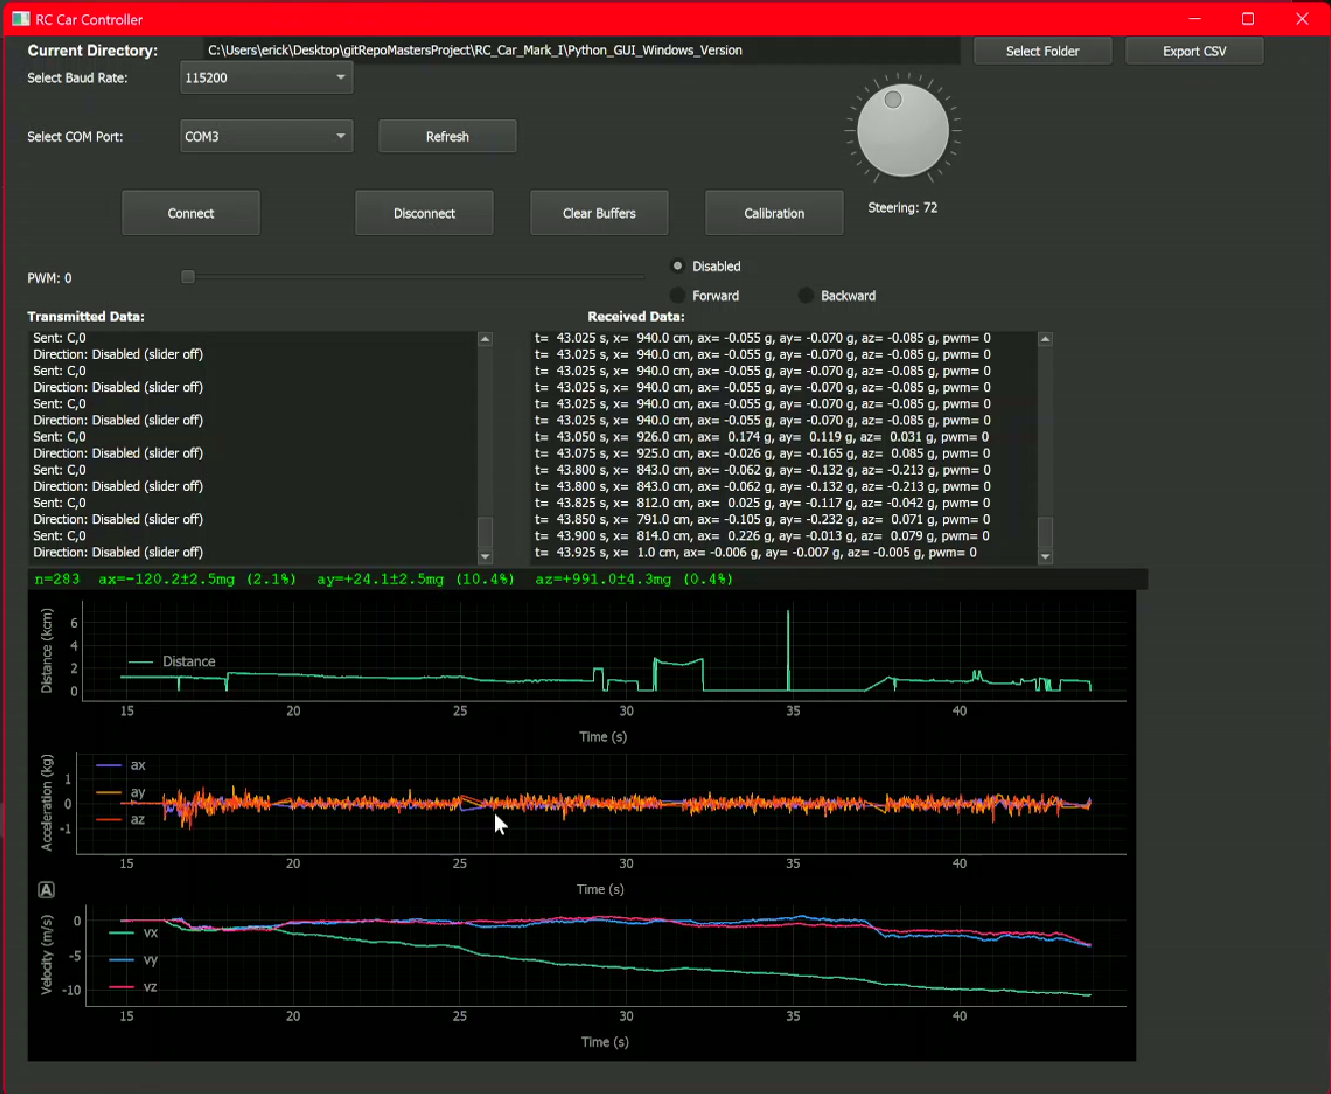
\includegraphics[width=0.7\textwidth]{docs/images/picturesGeneral/RC_Car_VidTestCalibration.png}
		\caption{The second test drive with the accelerometer calibrated.}
		\label{fig:CalibrationVidTest}
	\end{figure*}
	
	The velocity signal is calculated numerically using the Euler Integration
	Method as shown below, where $g$ is the acceleration due to gravity constant.
	
	\begin{equation}
		v_n = v_{n-1} + 0.001g \cdot a_n \cdot \Delta t
		\label{eq:euler}
	\end{equation}
	
	Since the sample rate of both sensors is 25ms, it can be assumed that this is
	sufficient for numerical integration. However, since the Z-axis component is
	consistently approximately 1g on average, the Z-axis velocity (shown in pink)
	increases over time, indicating that the RC Car appears to be falling for 30
	seconds, which is clearly not the case as shown in Figure~\ref{fig:TestDrive}.
	The zoomed plot shows the behavior of the accelerometer in the X and Y
	components, where the Y-axis velocity is close to zero. This indicates that
	the RC Car was not tilting sideways during the 30-second run, but the X-axis
	velocity at the 30-second mark suggests the car is constantly accelerating and
	has reached 50~m/s when the test stopped, which is not the case.
	
	The RC Car is tilted at an angle such that Earth's gravity influences the
	accelerometer X-axis component, which affects the X-axis velocity calculation
	as shown in the plotted signal. Since the accelerometer was theoretically
	intended to calculate the RC Car's velocity, an additional feature was added so
	that the gravitational influence can be filtered out. The Calibration button
	opens a separate window that samples the accelerometer data and calculates the
	DC bias, which represents the gravitational components. The mean and standard
	deviation are calculated so that the DC bias can be subtracted from subsequent
	accelerometer measurements.
	
	Figures~\ref{fig:NoCalibrationTest} and~\ref{fig:CalibrationTest} show the
	accelerometer waveforms for approximately 4 seconds while the RC Car is
	stationary. When calibrated, the accelerometer readings are close to 0mg for
	all X, Y, and Z axes, compared to the uncalibrated waveform. The mean and
	standard deviation are displayed in neon green text above the plots, which are
	the offset values subtracted from subsequent accelerometer measurements. The
	second video demonstrates the difference in velocity calculation compared to
	the uncalibrated version. Figure~\ref{fig:CalibrationVidTest} shows the second
	test drive with the offset values filtered from the measurements, where the
	measured values are more reasonable compared to the uncalibrated version.
	Although the velocity values are within a reasonable range, the signal still
	suffers from drift away from the true measurements, increasing over time due to
	accumulated noise.
	
	\begin{figure*}[t]
		\centering
		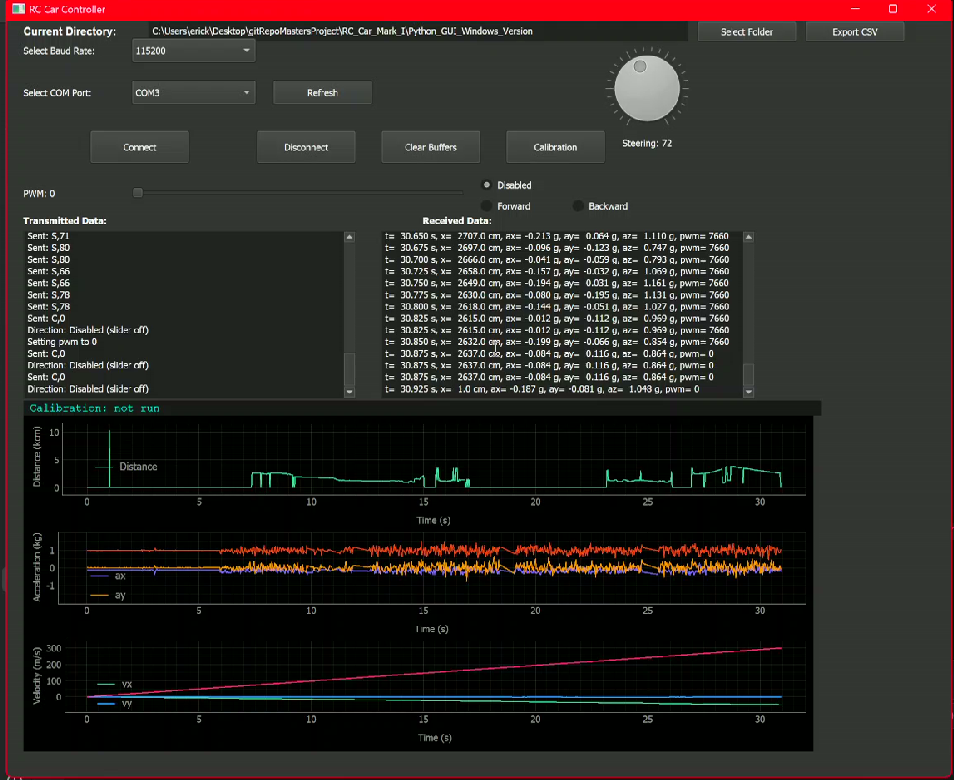
\includegraphics[width=0.7\textwidth]{docs/images/picturesGeneral/RC_Car_VidTestGUI.png}
		\caption{The User Interface during the 30-second test.}
		\label{fig:TestDrive}
	\end{figure*}
	
	\begin{figure*}[t]
		\centering
		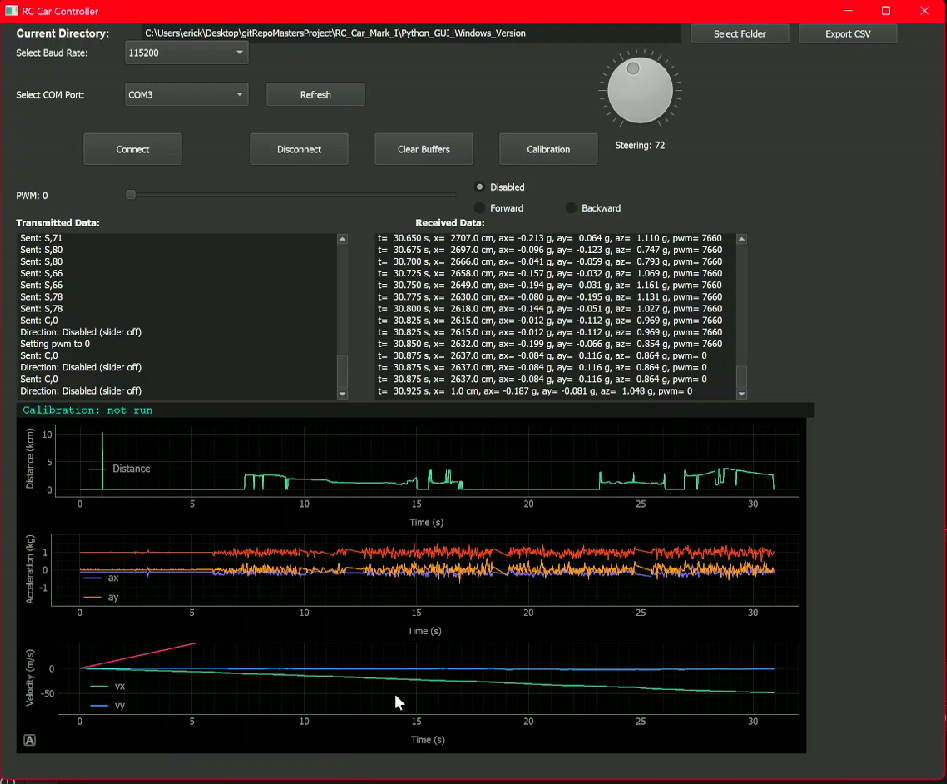
\includegraphics[width=0.7\textwidth]{docs/images/picturesGeneral/RC_Car_VidTestGUI_VelocityZoomed.png}
		\caption{The same User Interface with the X and Y velocity components zoomed in.}
		\label{fig:TestDriveZoomedVelocity}
	\end{figure*}
	
	\clearpage
	
	\begin{figure*}[t]
		\centering
		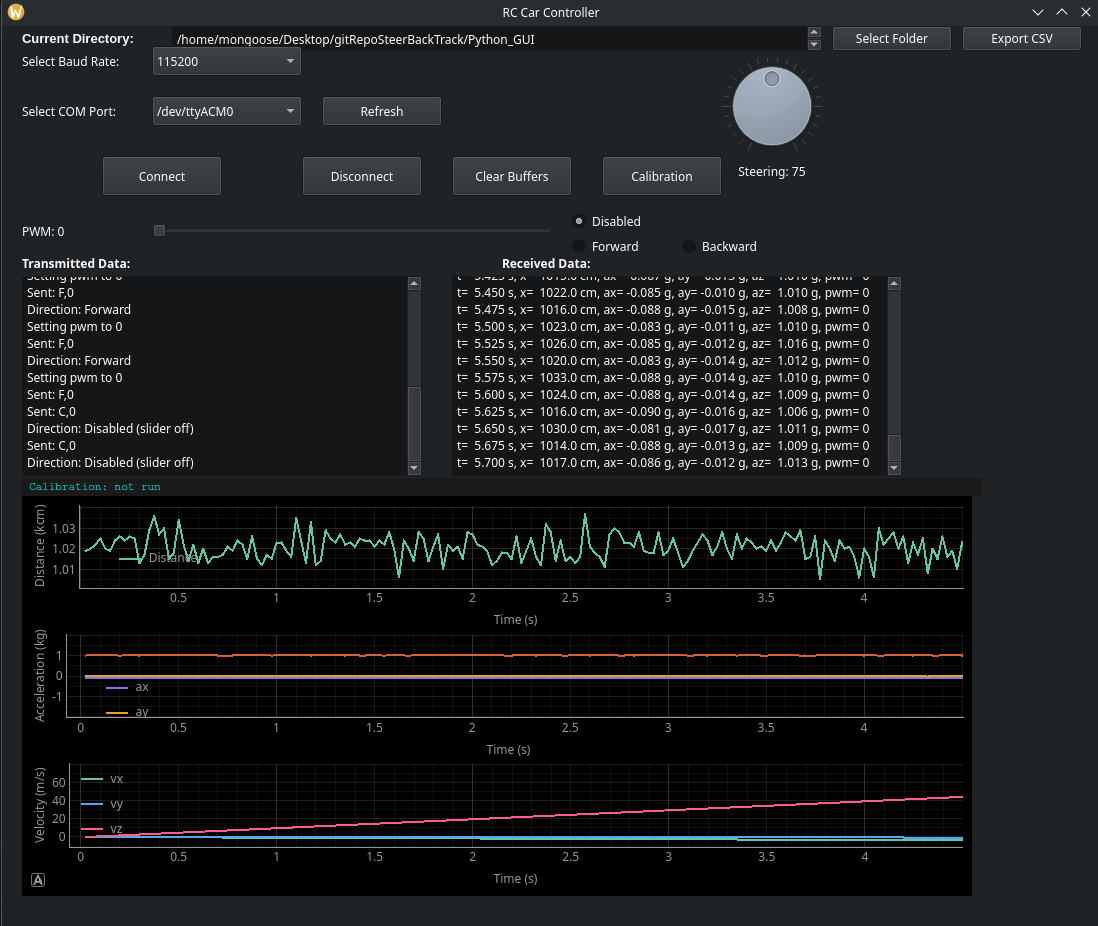
\includegraphics[width=0.7\textwidth]{docs/images/picturesGeneral/NoCalibrationWF.png}
		\caption{Accelerometer waveform without calibration.}
		\label{fig:NoCalibrationTest}
	\end{figure*}
	
	\begin{figure*}[t]
		\centering
		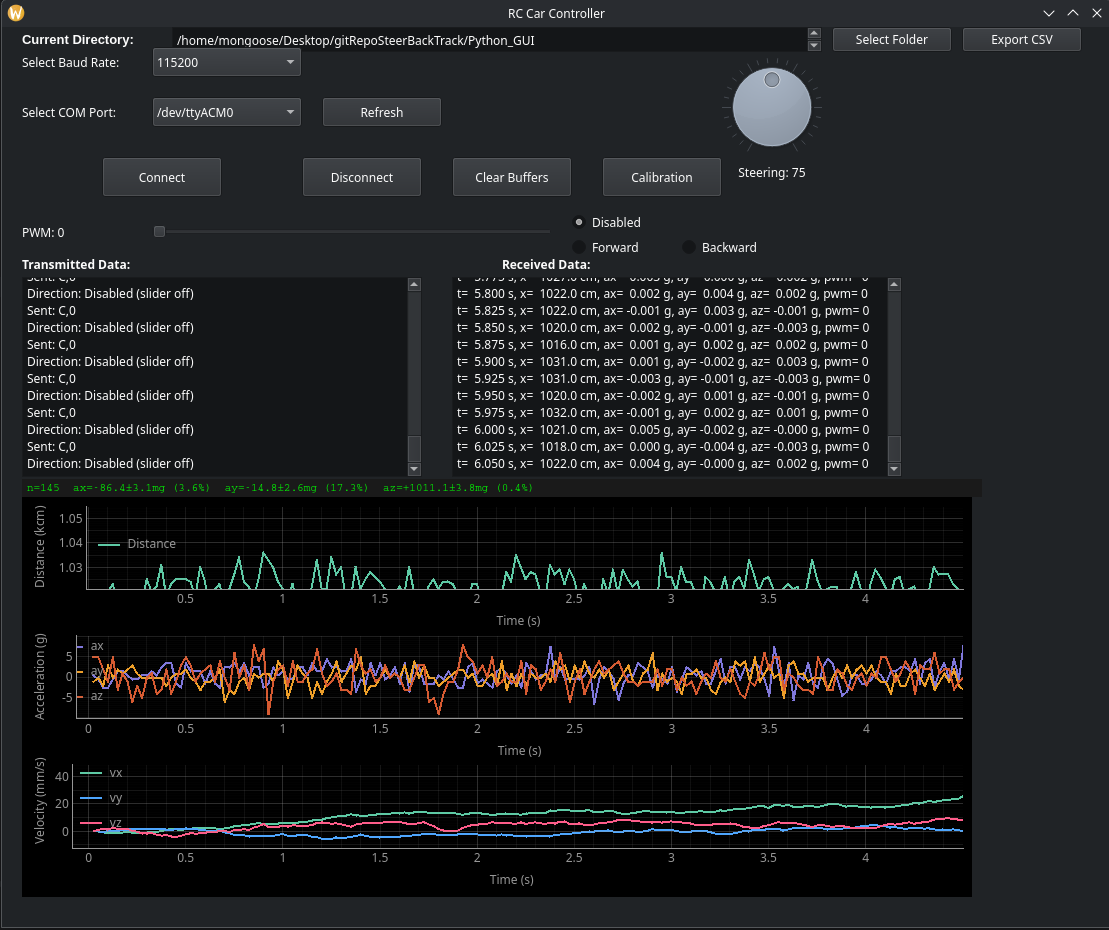
\includegraphics[width=0.7\textwidth]{docs/images/picturesGeneral/CalibrationWF.png}
		\caption{Accelerometer waveform with calibration applied.}
		\label{fig:CalibrationTest}
	\end{figure*}
	
	\clearpage
	
	% --- VI. Conclusion ----------------------------------------------------------
	\begin{figure*}[t]
		\centering
		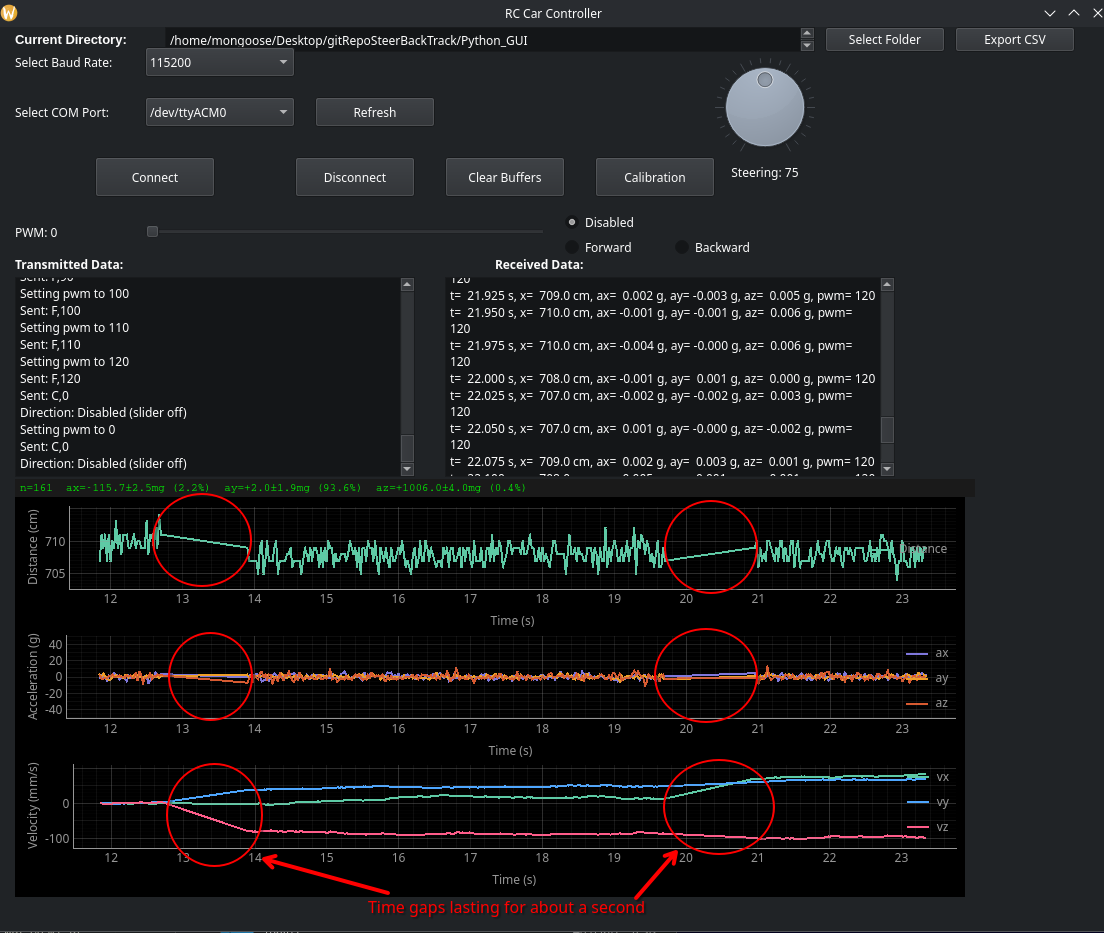
\includegraphics[width=0.7\textwidth]{docs/images/picturesGeneral/timeGapIssue.png}
		\caption{A sample waveform showing where time gaps occurred.}
		\label{fig:TimeGaps}
	\end{figure*}
	
	\section{Conclusion and Future Improvements}
	\label{sec:conclusion}
	
	The RC Car, Transmitter, and User Interface were successfully developed and the
	system was able to respond to commands and receive data through the user
	interface, though the adaptive cruise controller could not yet be fully
	implemented. Two factors affected the development of the adaptive cruise
	controller: inconsistent data acquisition sampling and the drifting effect from
	the velocity calculation. By addressing these two factors, there are potential
	improvements that can be made to obtain accurate measurements in real time.
	
	Data acquisition worked for most of the time but there are time gaps of lost
	data as shown in Figure~\ref{fig:TimeGaps}. This is due to the NRF24L01 on
	either the RC Car not transmitting, or the transmitter being in talk mode where
	it could not receive the data. Before integrating the steering mechanism, the
	system used to sample consistently without losing data. During testing, the RC
	Car crashed and weakened the socket where the NRF24L01 is placed. In the
	NRF24L01 library during data transmission from the RC Car to the transmitter, a
	red built-in status LED of the Nucleo-H723ZG board is toggled to indicate that
	data was packaged and transmitted; otherwise transmission is blocked if the red
	status LED does not toggle. Similarly, the transmitter toggles its status red
	LED to indicate that data was received. During the time gaps, the transmitter
	red LED does not toggle, which is a potential indication that it could not
	receive the data after the RC Car transmitted it. Since data collection used to
	be consistent, the NRF24L01 modules on both the RC Car and transmitter would
	need to be soldered directly to ensure good contact and prevent this issue from
	recurring. Another approach would be to probe the status red LEDs on a logic
	analyzer to determine whether the NRF24L01 is failing to configure TX/RX mode
	in time. Two of the FOD8001 logic optocouplers could be wired from both the RC
	Car and transmitter so that both signals share the same ground, making it
	easier to compare the time sequences during troubleshooting. With time gaps of
	lost communication lasting 1--1.5 seconds as shown in the waveform, this would
	drastically affect the velocity calculation. By resolving the time gap issue,
	the remaining challenge would be the drifting from the integration calculation.
	
	In theory, the accelerometer has the potential to measure the velocity of the
	RC Car, but in practice, drifting over time is a common issue for IMU sensors.
	Although calibration reduces most of the velocity error by removing the
	gravitational offsets measured by the accelerometer, it is a partial solution
	to the drift effect. Sensor noise plays a significant role in accumulating
	drift, as the accelerometer is well suited for detecting jolts (rapid changes
	in acceleration). When numerically integrating velocity, the calculation relies
	on acceleration data but does not know the initial condition of the RC Car at
	any given moment. For instance, the RC Car can run at a constant speed until it
	is signaled to stop. The accelerometer would detect the deceleration but would
	not be sufficient to confirm that the RC Car has stopped. At zero acceleration,
	the RC Car could be either stationary or moving at a constant speed, and the
	integration calculation does not know the initial condition at that moment. One
	proposal to address the drifting issue is sensor fusion, where additional
	sensors can be incorporated to describe more physical parameters of the RC Car.
	
	A magnet can be attached to the wheels and a Hall Effect sensor placed near the
	RC Car to measure the RPM, which can eventually be used to observe the velocity
	of the RC Car. The accelerometer could be supplemented or replaced with Hall
	Effect sensors, but at low RPM the timer may not be able to time the next pulse
	from the Hall Effect sensor since the timer resets when $2^{16}$ or $2^{32}$
	ticks have passed. The accelerometer and Hall Effect sensor can be fused so
	that the system has the initial conditions needed when calculating velocity,
	providing a better description of the physical state of the RC Car compared to
	the accelerometer data alone. This is a precursor to Kalman Filters, which can
	be implemented to compare the observed measurement and predicted measurement so
	that when integration is performed it can correct itself when drift occurs. The
	mathematics of Kalman Filters can be explored in order to properly implement
	this approach so that measurements become accurate and reliable enough to
	develop the adaptive cruise controller.
	
	% --- References --------------------------------------------------------------
	\begin{thebibliography}{9}
		
		\bibitem{stm32h723}
		STMicroelectronics, \textit{STM32H723ZG Datasheet}, Rev.~4, 2022. [Online].
		Available: \url{https://www.st.com/resource/en/datasheet/stm32h723zg.pdf}
		[Accessed: May 2026].
		
		\bibitem{stm32l432}
		STMicroelectronics, \textit{STM32L432KC Datasheet}, Rev.~7, 2021. [Online].
		Available: \url{https://www.st.com/resource/en/datasheet/stm32l432kc.pdf}
		[Accessed: May 2026].
		
		\bibitem{lis3dh}
		STMicroelectronics, \textit{LIS3DH Datasheet}, Rev.~3, 2016. [Online]. 
		Available: \url{https://www.st.com/resource/en/datasheet/lis3dh.pdf}
		[Accessed: May 2026].
		
		\bibitem{nrf24l01}
		Nordic Semiconductor, \textit{nRF24L01+ Single Chip 2.4GHz Transceiver 
			Product Specification}, Rev.~1.0, 2008. [Online]. Available:
		\url{https://www.nordicsemi.com/products/nrf24l01}
		[Accessed: May 2026].
		
		\bibitem{lidar}
		Garmin Ltd., \textit{LIDAR-Lite v3 Operation Manual}, 2017. [Online].
		Available: \url{https://static.garmin.com/pumac/LIDAR_Lite_v3_Operation_Manual_and_Technical_Specifications.pdf}
		[Accessed: May 2026].
		
		\bibitem{mathworks_acc}
		MathWorks, ``Adaptive Cruise Control Using Model Predictive Controller,''
		\textit{MATLAB Documentation}, 2024. [Online]. Available:
		\url{https://www.mathworks.com/help/mpc/ug/adaptive-cruise-control-using-model-predictive-controller.html}
		[Accessed: May 2026].
		
	\end{thebibliography}
	
	% --- Code Availability -------------------------------------------------------
	\section*{Code Availability}
	
	The complete firmware, Python GUI source code, schematics, and documentation 
	for this project are publicly available on GitHub:
	\url{https://github.com/eam95/RC_Car_Mark_I}
	
	\bigskip
	
\end{document}